%%%%%%%%%%%%%%%%% ASYLUM original card game

%Renaud Dubois: creator and game designer, artistic lead
%Aurélien Dupin: technical director



\documentclass[parskip]{scrartcl}
\usepackage[utf8]{inputenc}
\usepackage[T1]{fontenc}
\usepackage[paperheight=96mm,paperwidth=71mm,margin=0mm]{geometry}
\usepackage{xintexpr}
\usepackage{tikz}
\usetikzlibrary{positioning}
\usetikzlibrary{shapes.arrows}
\usetikzlibrary{fadings}
\usepackage{pifont}
\usepackage{graphicx}
\usepackage{xfp}
\usepackage{ifthen}
\usepackage{atbegshi}
\AtBeginDocument{\AtBeginShipoutNext{\AtBeginShipoutDiscard}} %pour supprimer la premiere page

\DeclareOldFontCommand{\bf}{\normalfont\bfseries}{\mathbf}

\begin{document}

\pgfmathsetmacro{\cardroundingradius}{4mm}
\pgfmathsetmacro{\cardwidth}{6.8}
\pgfmathsetmacro{\cardheight}{9.3}

\pgfmathsetmacro{\titleX}{3.55}
\pgfmathsetmacro{\titleY}{8.7}
\pgfmathsetmacro{\imageX}{3.555}
\pgfmathsetmacro{\imageY}{6.32}
\pgfmathsetmacro{\typeX}{3.55}
\pgfmathsetmacro{\typeY}{4}
\pgfmathsetmacro{\imageWidth}{159}
\pgfmathsetmacro{\imageHeight}{115}
\pgfmathsetmacro{\descriptionX}{.63}
\pgfmathsetmacro{\descriptionY}{3.7}
%\pgfmathsetmacro{\punchlineX}{.5}
%\pgfmathsetmacro{\punchlineY}{1.8}
\pgfmathsetmacro{\numberX}{5.8}
\pgfmathsetmacro{\numberY}{.94}

\renewcommand{\titlefont}{}
\newcommand{\typefont}{\bf}
\newcommand{\punchlinefont}{\itshape}
\newcommand{\descriptionfont}{}
\newcommand{\numberfont}{}
\newcommand{\setsize}[1]{\fontsize{#1pt}{\fpeval{1*(#1)}pt}\selectfont}

\newcounter{cardctr}
\newcommand{\cardnumber}{\stepcounter{cardctr}\thecardctr\ifthenelse{\equal{\thecardctr}{8}}{\setcounter{cardctr}{0}}{}}

%VersoPerso
\newcommand{\versoperso}{ %TODO A recentrer et elargir
\begin{tikzpicture}
    \node[anchor=south west,inner sep=0] at (0,0) {
\includegraphics[width=7.1 cm, height=9.6 cm]{fonds/versoperso.pdf}};
\end{tikzpicture}}

%Verso
\newcommand{\verso}{ %TODO A recentrer et elargir
\begin{tikzpicture}
    \node[anchor=south west,inner sep=0] at (0,0) {
\includegraphics[width=7.1 cm, height=9.6 cm]{fonds/verso.pdf}};
\end{tikzpicture}}


%DEBUT DU DOCUMENT


%--------------------------CARTES PERSONNAGE--------------------------------------------------------------------------------------------
%!TEX root = lot1.tex
%--------------------------CARTES PERSONNAGE--------------------------------------------------------------------------------------------

\begin{tikzpicture} %Recto
	%Fond
    \node[anchor=south west,inner sep=0] (carte) at (0,0) {
\includegraphics[width=7.1 cm, height=9.6 cm]{fonds/noir.png}};
    \node[anchor=center] at (carte.center) {
\includegraphics[width=\cardwidth cm, height=\cardheight cm]{fonds/fond_plan.png}};

    %Titre
	\node[anchor=center] at (\titleX,\titleY) {\titlefont Planning};

	%Description
	\node[anchor=north west, text width=5.6cm] (description) at (\descriptionX,8) {\descriptionfont\setsize{11} \begin{enumerate}
\item DSI
\item Stagiaire
\item Manager
\item Marketing
\item PMO
\item Développeur
\item Cryptologue
\item Ingénieur Système
\item {\textit{ Assistante de Direction}}
\end{enumerate}
};

\end{tikzpicture}

\begin{tikzpicture} %Verso
	%Fond
    \node[anchor=south west,inner sep=0] (carte) at (0,0) {
\includegraphics[width=7.1 cm, height=9.6 cm]{fonds/noir.png}};
    \node[anchor=center] at (carte.center) {
\includegraphics[width=\cardwidth cm, height=\cardheight cm]{fonds/fond_plan.png}};

    %Titre
	\node[anchor=center] at (\titleX,\titleY) {\titlefont Planning};

	%Description
	\node[anchor=north west, text width=5.6cm] (description) at (\descriptionX,8) {\descriptionfont\setsize{11} \begin{enumerate}
\item DSI
\item Stagiaire
\item Manager
\item Marketing
\item PMO
\item Développeur
\item Cryptologue
\item Ingénieur Système
\item {\textit {Assistante de Direction}}
\end{enumerate}
};

\end{tikzpicture}



%%%%%%%%%%%%%%%%%%%%%%%%%%%%%%%%%%%%%%%%%%%%%%%%%%%%%%%%%%%%%%

\begin{tikzpicture} %Recto
	%Fond
    \node[anchor=south west,inner sep=0] (carte) at (0,0) {
\includegraphics[width=7.1 cm, height=9.6 cm]{fonds/noir.png}};
    \node[anchor=center] at (carte.center) {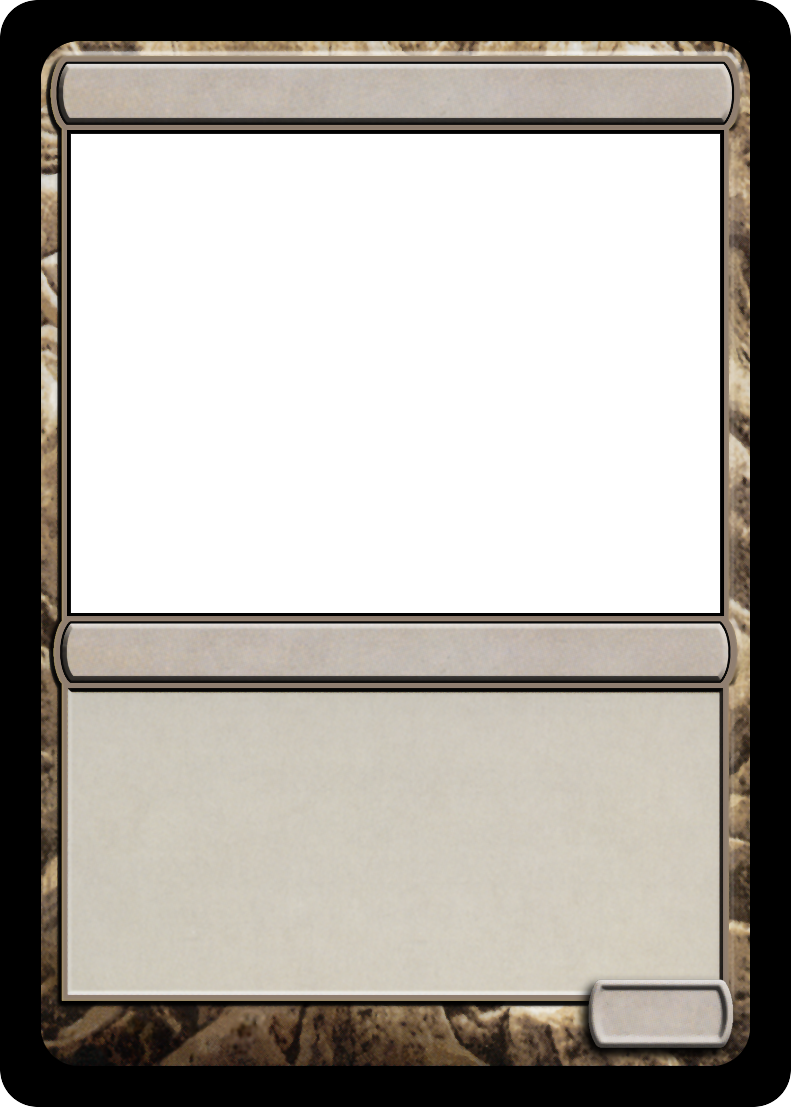
\includegraphics[width=\cardwidth cm, height=\cardheight cm]{fonds/fond_personnage.png}};

    %Titre
	\node[anchor=center] at (\titleX,\titleY) {\titlefont DSI};

	%Image
	\node[anchor=center] at (\imageX,\imageY) {
\includegraphics[width=\imageWidth px, height=\imageHeight px]{images/P1_DSI.png}};
	\node[anchor=center] at (6.1,4.5) {
\includegraphics[width=12 px, height=6 px]{fonds2/legacy.jpg}};

	%Type
	\node[anchor=center] at (\typeX,\typeY) {\typefont Personnage};

	%Description
	\node[anchor=north west, text width=5.6cm] (description) at (\descriptionX,\descriptionY) {\descriptionfont\setsize{6}(Bonus) DSI paralyse un personnage pour ce tour. Le joueur terminera son UO directement sans piocher. Celui-ci doit également écrire le mot ``demande KiSS'' sur un papier pendant que les autres jouent leur UO. Le joueur DSI jettera avec le plus grand mépris la demande à la poubelle.\par};

	%Punchline
	\node[anchor=north west, text width=5.6cm, below = 1pt of description] (punchline) {\punchlinefont\setsize{6}(Permanent) Avant de vous parler, les autres joueurs doivent dire 3915.\par};

	%Separateur !!!!!PAS TOUCHE!!!!!
	\fill[black,path fading=west] (description.south west) rectangle (punchline.north);
	\fill[black,path fading=east] (punchline.north) rectangle (description.south east);

	%Numéro !!!!!PAS TOUCHE!!!!!
	\node[anchor=center] at (\numberX,\numberY) {\numberfont 1/8};
\end{tikzpicture}\versoperso %Verso

%%%%%%%%%%%%%%%%%%%%%%STAGIAIRE%%%%%%%%%%%%%%%%%%%%%%%%%%%%%%%%%%%%%%%%
\begin{tikzpicture} %Recto
	%Fond
    \node[anchor=south west,inner sep=0] (carte) at (0,0) {
\includegraphics[width=7.1 cm, height=9.6 cm]{fonds/noir.png}};
    \node[anchor=center] at (carte.center) {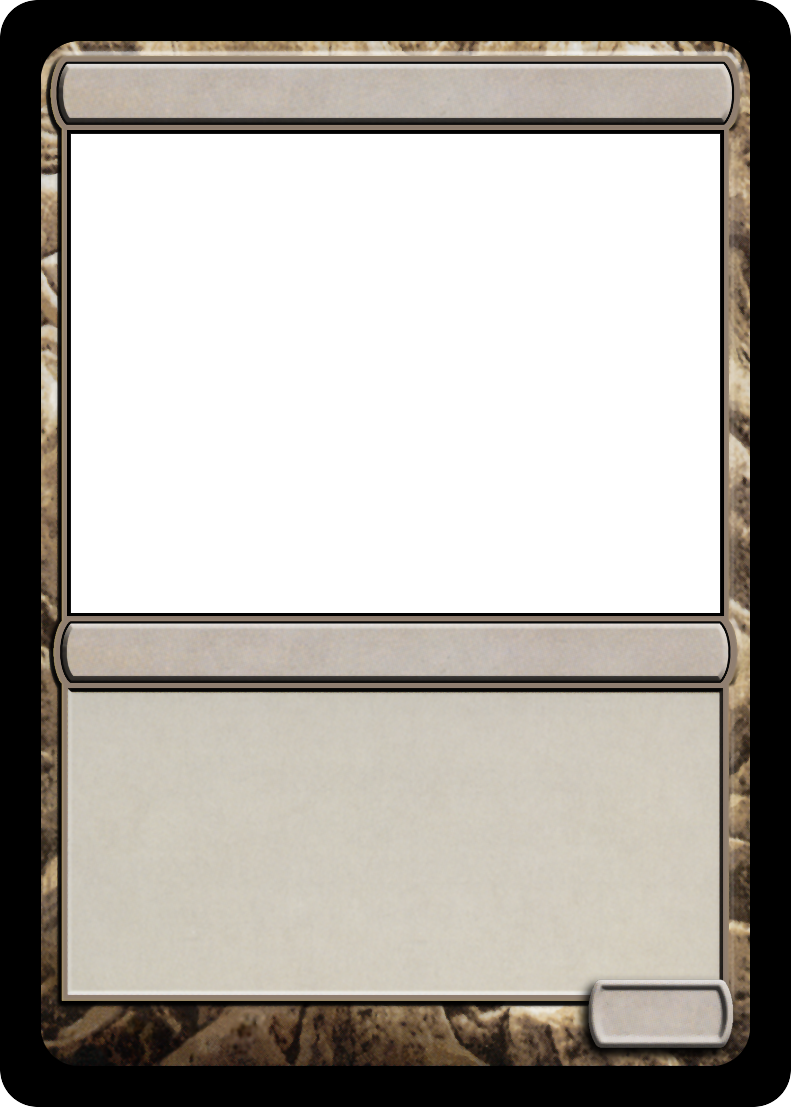
\includegraphics[width=\cardwidth cm, height=\cardheight cm]{fonds/fond_personnage.png}};

    %Titre
	\node[anchor=center] at (\titleX,\titleY) {\titlefont Stagiaire};

	%Image
	\node[anchor=center] at (\imageX,\imageY) {
\includegraphics[width=\imageWidth px, height=\imageHeight px]{images/P2_Stagiaire.jpg}};
	\node[anchor=center] at (6.1,4.5) {
\includegraphics[width=12 px, height=6 px]{fonds2/legacy.jpg}};

	%Type
	\node[anchor=center] at (\typeX,\typeY) {\typefont Personnage};

	%Description
	\node[anchor=north west, text width=5.6cm] (description) at (\descriptionX,\descriptionY) {\descriptionfont\setsize{6}(Bonus) Le stagiaire choisit un joueur autour de la table qui sera son tuteur. Il tire un CDI à pile ou face. En cas de victoire il obtient un tour supplémentaire `nouveau contrat' à la fin du tour avec effet bonus équivalent à celui du tuteur.\par};

	%Punchline
	\node[anchor=north west, text width=5.6cm, below = 1pt of description] (punchline) {\punchlinefont\setsize{5}(Invisibilité) Seul le tuteur peut jouer des cartes malus contre lui. Son tuteur peut lui demander d’aller chercher un café pendant le tour. Les autres joueurs vous appellent ``machin''.\par};

	%Separateur !!!!!PAS TOUCHE!!!!!
	\fill[black,path fading=west] (description.south west) rectangle (punchline.north);
	\fill[black,path fading=east] (punchline.north) rectangle (description.south east);

	%Numéro !!!!!PAS TOUCHE!!!!!
	\node[anchor=center] at (\numberX,\numberY) {\numberfont 2/8};
\end{tikzpicture}\versoperso %Verso

%%%%%%%%%%%%%%%%%%%%%%%%%%%%%%%%%%%%%%%%%%%%%%%%%%%%%%%%%%%%%%

\begin{tikzpicture} %Recto
	%Fond
    \node[anchor=south west,inner sep=0] (carte) at (0,0) {
\includegraphics[width=7.1 cm, height=9.6 cm]{fonds/noir.png}};
    \node[anchor=center] at (carte.center) {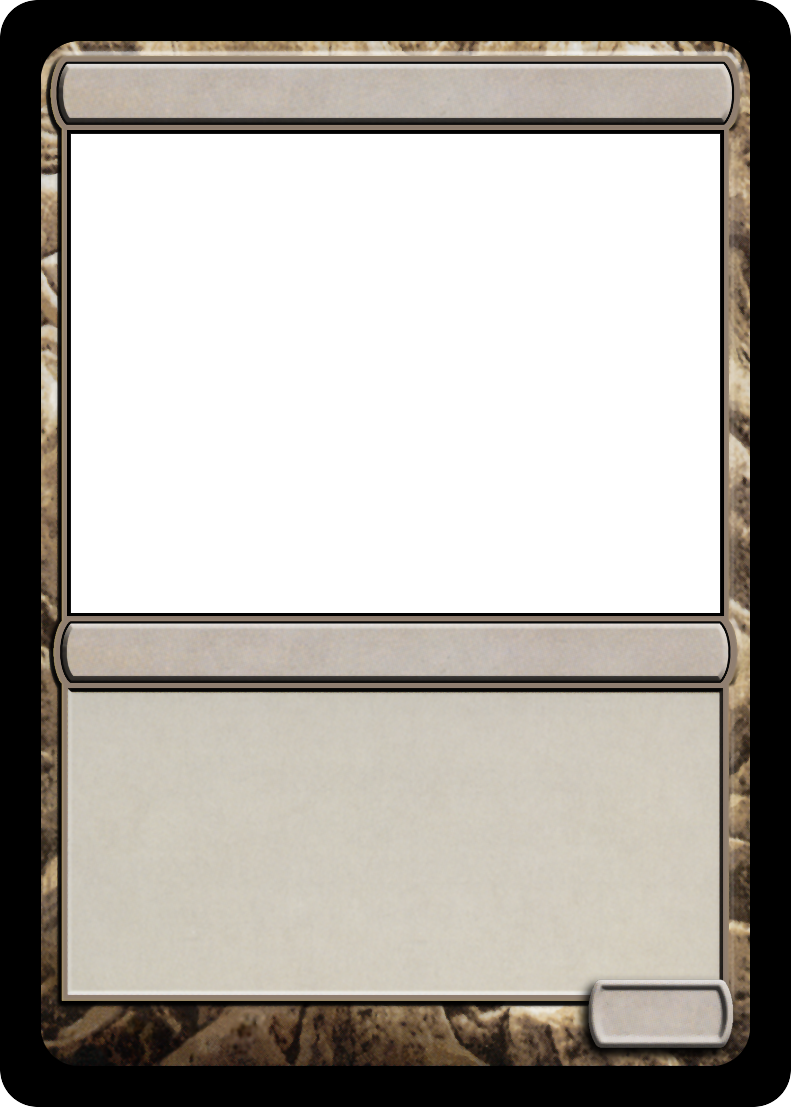
\includegraphics[width=\cardwidth cm, height=\cardheight cm]{fonds/fond_personnage.png}};

    %Titre
	\node[anchor=center] at (\titleX,\titleY) {\titlefont Manager};

	%Image
	\node[anchor=center] at (\imageX,\imageY) {
\includegraphics[width=\imageWidth px, height=\imageHeight px]{images/P3_Manager.jpg}};
	\node[anchor=center] at (6.1,4.5) {
\includegraphics[width=12 px, height=6 px]{fonds2/legacy.jpg}};

	%Type
	\node[anchor=center] at (\typeX,\typeY) {\typefont Personnage};

	%Description
	\node[anchor=north west, text width=5.6cm] (description) at (\descriptionX,\descriptionY) {\descriptionfont\setsize{6}(Délégation) Il peut déléguer une carte de sa main vers un autre personnage de son choix et demander à un joueur d’échanger sa chaise avec un autre. \par};

	%Punchline
	\node[anchor=north west, text width=5.6cm, below = 1pt of description] (punchline) {\punchlinefont\setsize{6}(Directisation) Lorsqu’un joueur peut défausser une carte, révéler une carte, si elle vaut 8 vous directisez (défaussez) à la place du joueur. Les autres joueurs doivent appeler le personnage ``chef''. \par};

	%Separateur !!!!!PAS TOUCHE!!!!!
	\fill[black,path fading=west] (description.south west) rectangle (punchline.north);
	\fill[black,path fading=east] (punchline.north) rectangle (description.south east);

	%Numéro !!!!!PAS TOUCHE!!!!!
	\node[anchor=center] at (\numberX,\numberY) {\numberfont 3/8};
\end{tikzpicture}\versoperso %Verso

%%%%%%%%%%%%%%%%%%%%%%%%%%%%%%%%%%%%%%%%%%%%%%%%%%%%%%%%%%%%%% MARKET
\begin{tikzpicture} %Recto
	%Fond
    \node[anchor=south west,inner sep=0] (carte) at (0,0) {
\includegraphics[width=7.1 cm, height=9.6 cm]{fonds/noir.png}};
    \node[anchor=center] at (carte.center) {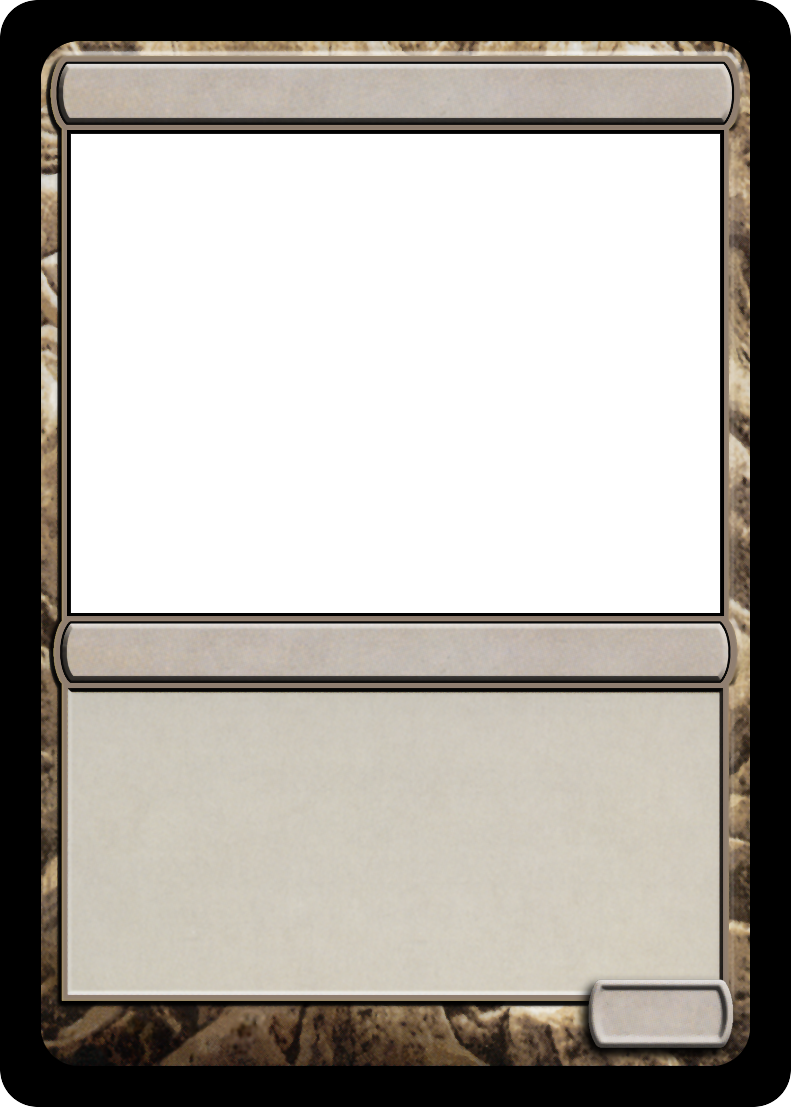
\includegraphics[width=\cardwidth cm, height=\cardheight cm]{fonds/fond_personnage.png}};

    %Titre
	\node[anchor=center] at (\titleX,\titleY) {\titlefont Marketing};

	%Image
	\node[anchor=center] at (\imageX,\imageY) {
\includegraphics[width=\imageWidth px, height=\imageHeight px]{images/P4_Marketting.jpg}};
	\node[anchor=center] at (6.1,4.5) {
\includegraphics[width=12 px, height=6 px]{fonds2/legacy.jpg}};

	%Type
	\node[anchor=center] at (\typeX,\typeY) {\typefont Personnage};

	%Description
	\node[anchor=north west, text width=5.6cm] (description) at (\descriptionX,\descriptionY) {\descriptionfont\setsize{6}(Enfumage) Le marketing peut en*u*er$^1$ le personnage de son choix et échanger jusqu’à 4 cartes de sa main avec des cartes choisies aléatoirement dans celle d’un autre joueur.\par};

	%Punchline
	\node[anchor=north west, text width=5.6cm, below = 1pt of description] (punchline) {\punchlinefont\setsize{6}(Permanent) Les autres joueurs vous méprisent techniquement, mais sont jaloux de vous.\par};

	%Specifique à cette carte
	\node[anchor=north west, text width=5.6cm, below = 1pt of punchline] (footnote) {\descriptionfont\setsize{5}1 : enfumer évidemment. Pervers !\par};

	%Separateur !!!!!PAS TOUCHE!!!!!
	\fill[black,path fading=west] (description.south west) rectangle (punchline.north);
	\fill[black,path fading=east] (punchline.north) rectangle (description.south east);

	%Numéro !!!!!PAS TOUCHE!!!!!
	\node[anchor=center] at (\numberX,\numberY) {\numberfont 4/8};
\end{tikzpicture}\versoperso %Verso

%%%%%%%%%%%%%%%%%%%%%%%%%%%%%%%%%%%%%%%%%%%%%%%%%%%%%%%%%%%%%% PMO
\begin{tikzpicture} %Recto
	%Fond
    \node[anchor=south west,inner sep=0] (carte) at (0,0) {
\includegraphics[width=7.1 cm, height=9.6 cm]{fonds/noir.png}};
    \node[anchor=center] at (carte.center) {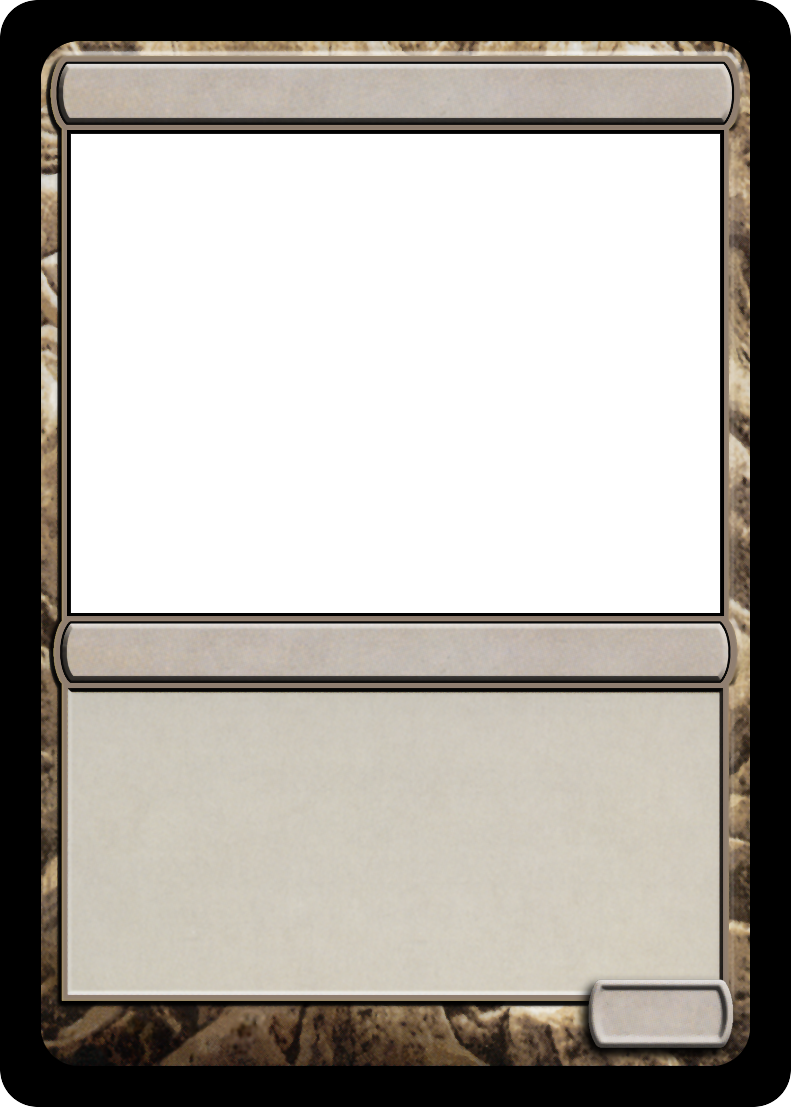
\includegraphics[width=\cardwidth cm, height=\cardheight cm]{fonds/fond_personnage.png}};

    %Titre
	\node[anchor=center] at (\titleX,\titleY) {\titlefont PMO (Gestionnaire)};

	%Image
	\node[anchor=center] at (\imageX,\imageY) {
\includegraphics[width=\imageWidth px, height=\imageHeight px]{images/P5_pmo.jpg}};
	\node[anchor=center] at (6.1,4.5) {
\includegraphics[width=12 px, height=6 px]{fonds2/legacy.jpg}};

	%Type
	\node[anchor=center] at (\typeX,\typeY) {\typefont Personnage ennuyeux};

	%Description
	\node[anchor=north west, text width=5.6cm] (description) at (\descriptionX,\descriptionY) {\descriptionfont\setsize{8}(Planification) Le PMO acquiert la carte planning. Il peut jouer une carte neutre supplémentaire.\par};

	%Punchline
	\node[anchor=north west, text width=5.6cm, below = 1pt of description] (punchline) {\punchlinefont\setsize{8}(Permanent) Les autres joueurs ne vous écoutent pas attentivement durant ce tour.\par};

	%Separateur !!!!!PAS TOUCHE!!!!!
	\fill[black,path fading=west] (description.south west) rectangle (punchline.north);
	\fill[black,path fading=east] (punchline.north) rectangle (description.south east);

	%Numéro !!!!!PAS TOUCHE!!!!!
	\node[anchor=center] at (\numberX,\numberY) {\numberfont 5/8};
\end{tikzpicture}\versoperso %Verso

%%%%%%%%%%%%%%%%%%%%%%%%%%%% PERSONNAGE ELECTRONICIEN
\begin{tikzpicture} %Recto
	%Fond
    \node[anchor=south west,inner sep=0] (carte) at (0,0) {
\includegraphics[width=7.1 cm, height=9.6 cm]{fonds/noir.png}};
    \node[anchor=center] at (carte.center) {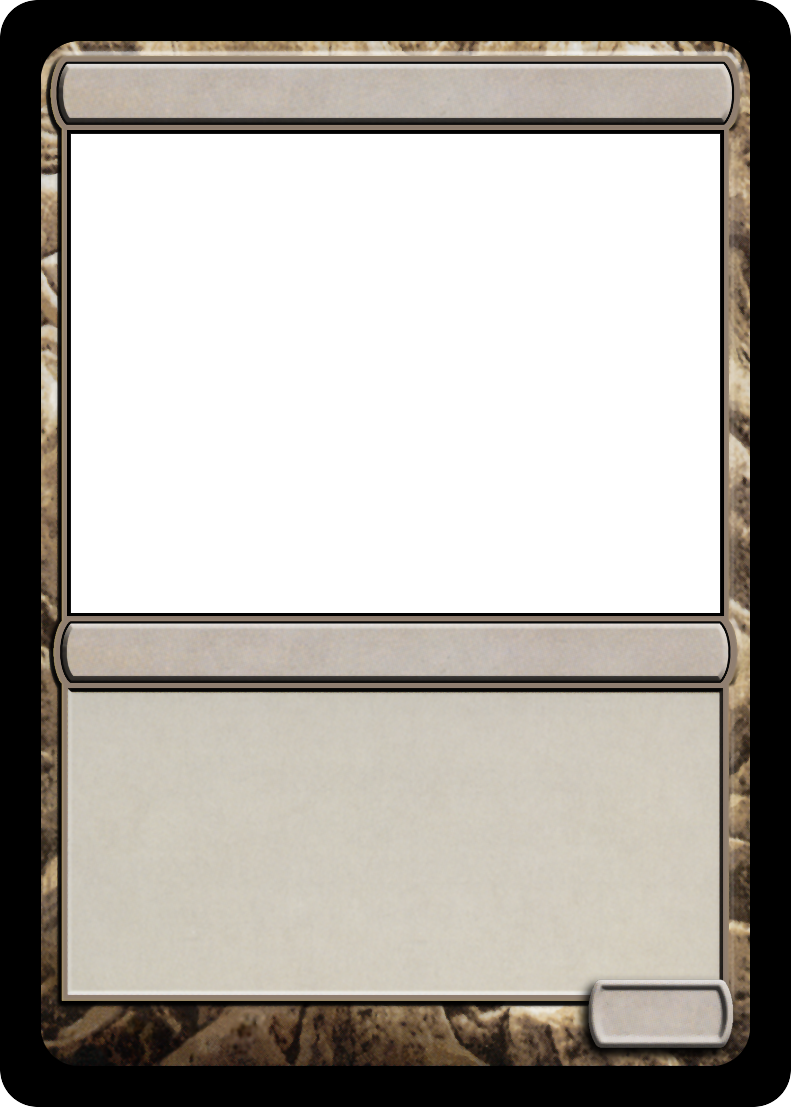
\includegraphics[width=\cardwidth cm, height=\cardheight cm]{fonds/fond_personnage.png}};

    %Titre
	\node[anchor=center] at (\titleX,\titleY) {\titlefont Composant (\'Electronicien) };

	%Image
	\node[anchor=center] at (\imageX,\imageY) {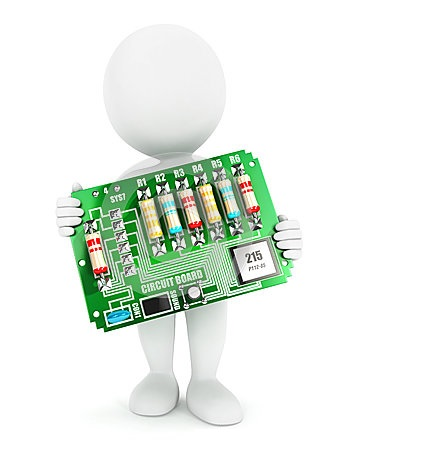
\includegraphics[width=\imageWidth px, height=\imageHeight px]{images/P9_compo.png}};
	\node[anchor=center] at (6.1,4.5) {
\includegraphics[width=12 px, height=6 px]{fonds2/legacy.jpg}};

	%Type
	\node[anchor=center] at (\typeX,\typeY) {\typefont Personnage };

	%Description
	\node[anchor=north west, text width=5.6cm] (description) at (\descriptionX,\descriptionY) {\descriptionfont\setsize{6}(VHDL) Le joueur dessine des petits créneaux sur une feuille puis révèle une carte du tas. En cas de parité identique avec le nombre de créneaux, le routage fonctionne et le personnage peut imputer deux cartes supplémentaires. \par};

	%Punchline
	\node[anchor=north west, text width=5.6cm, below = 1pt of description] (punchline) {\punchlinefont\setsize{6}(Outre-espace) Vous vivez aux confins lointains de la zone et devez vous asseoir à l'opposé de la table par rapport au cryptologue à ce tour.\par};

	%Separateur !!!!!PAS TOUCHE!!!!!
	\fill[black,path fading=west] (description.south west) rectangle (punchline.north);
	\fill[black,path fading=east] (punchline.north) rectangle (description.south east);

	%Numéro !!!!!PAS TOUCHE!!!!!
	\node[anchor=center] at (\numberX,\numberY) {\numberfont 6/8};
\end{tikzpicture}\versoperso %Verso

%%%%%%%%%%%%%%%%%%%%%%%%%%%%%%%%%%%%%%%%%%%%%%%%%%%%%%%%%%%%%% 7: CRYPTOLOGUE
\begin{tikzpicture} %Recto
	%Fond
    \node[anchor=south west,inner sep=0] (carte) at (0,0) {
\includegraphics[width=7.1 cm, height=9.6 cm]{fonds/noir.png}};
    \node[anchor=center] at (carte.center) {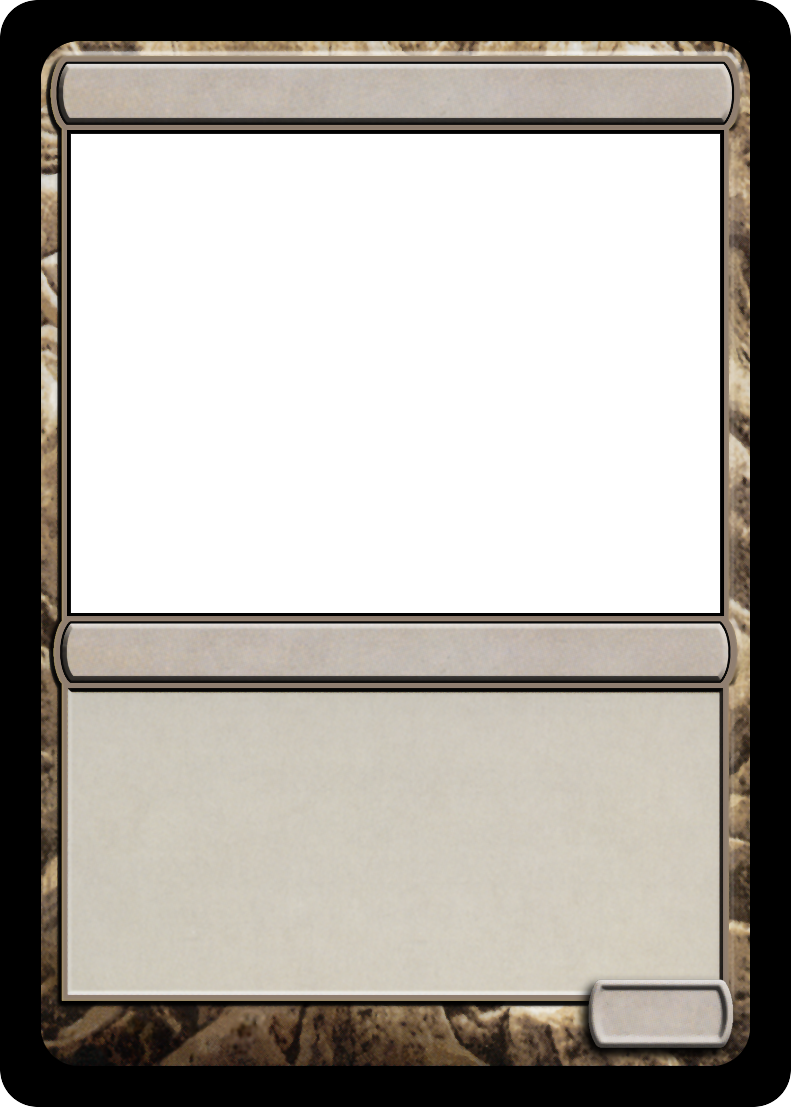
\includegraphics[width=\cardwidth cm, height=\cardheight cm]{fonds/fond_personnage.png}};

    %Titre
	\node[anchor=center] at (\titleX,\titleY) {\titlefont Cryptologue};

	%Image
	\node[anchor=center] at (\imageX,\imageY) {
\includegraphics[width=\imageWidth px, height=\imageHeight px]{images/P7_Cryptologue.jpg}};
	\node[anchor=center] at (6.1,4.5) {
\includegraphics[width=12 px, height=6 px]{fonds2/legacy.jpg}};

	%Type
	\node[anchor=center] at (\typeX,\typeY) {\typefont Personnage};

	%Description
	\node[anchor=north west, text width=5.6cm] (description) at (\descriptionX,\descriptionY) {\descriptionfont\setsize{8}(Astucieux) Le cryptologue pioche deux cartes puis défausse deux cartes. Il peut également imputer une carte supplémentaire.\par};

	%Punchline
	\node[anchor=north west, text width=5.6cm, below = 1pt of description] (punchline) {\punchlinefont\setsize{8}(Génial) Les autres joueurs vous admirent secrètement durant ce tour. \par};

	%Separateur !!!!!PAS TOUCHE!!!!!
	\fill[black,path fading=west] (description.south west) rectangle (punchline.north);
	\fill[black,path fading=east] (punchline.north) rectangle (description.south east);

	%Numéro !!!!!PAS TOUCHE!!!!!
	\node[anchor=center] at (\numberX,\numberY) {\numberfont 7/8};
\end{tikzpicture}\versoperso %Verso

%%%%%%%%%%%%%%%%%%%%%%%%%%%%%%%%%%%%%%%%%%%%%%%%%%%%%%%%%%%%%% 8: IS
\begin{tikzpicture} %Recto
	%Fond
    \node[anchor=south west,inner sep=0] (carte) at (0,0) {
\includegraphics[width=7.1 cm, height=9.6 cm]{fonds/noir.png}};
    \node[anchor=center] at (carte.center) {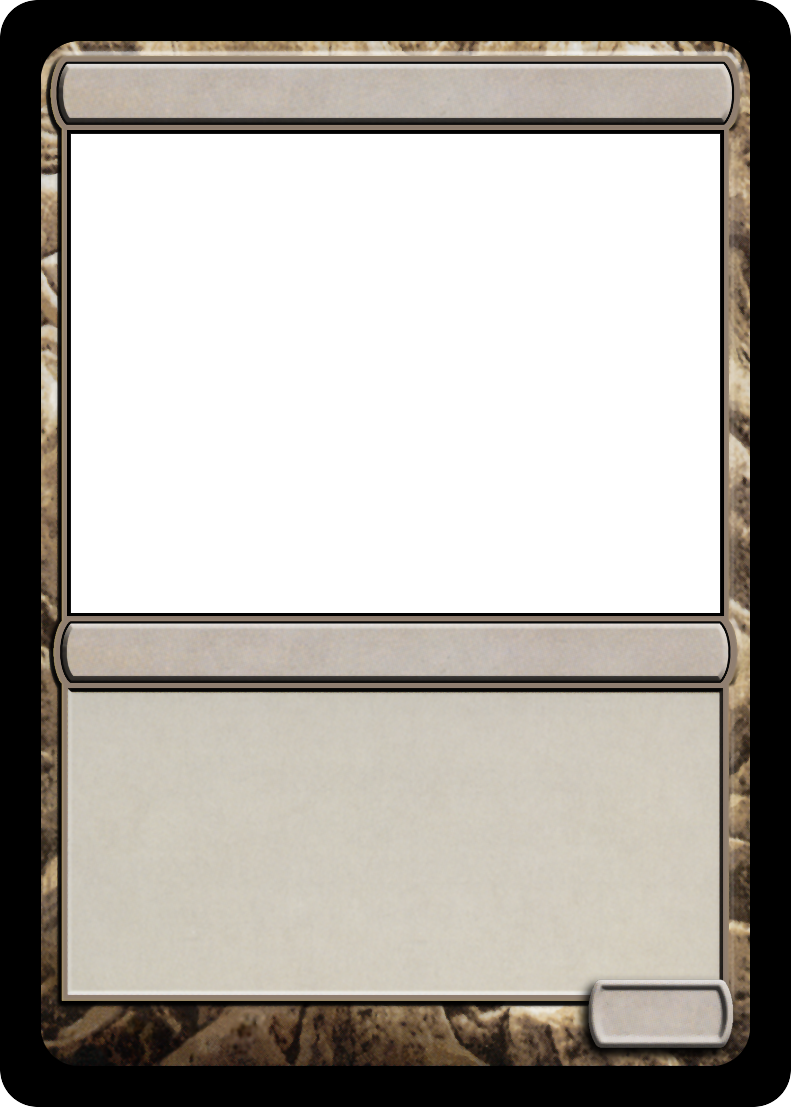
\includegraphics[width=\cardwidth cm, height=\cardheight cm]{fonds/fond_personnage.png}};

    %Titre
	\node[anchor=center] at (\titleX,\titleY) {\titlefont Ingénieur Système};

	%Image
	\node[anchor=center] at (\imageX,\imageY) {
\includegraphics[width=\imageWidth px, height=\imageHeight px]{images/P8_IS.png}};
	\node[anchor=center] at (6.1,4.5) {
\includegraphics[width=12 px, height=6 px]{fonds2/legacy.jpg}};

	%Type
	\node[anchor=center] at (\typeX,\typeY) {\typefont Personnage};

	%Description
	\node[anchor=north west, text width=5.6cm] (description) at (\descriptionX,\descriptionY) {\descriptionfont\setsize{8}(Bonus) Au début de son tour l’ingénieur système force un autre joueur de son choix à piocher une carte. L’ingénieur système remet toujours tout en cause et peut jouer une carte malus (ou côté spécifique malus) supplémentaire.\par};

	%Punchline
	\node[anchor=north west, text width=5.6cm, below = 1pt of description] (punchline) {\punchlinefont\setsize{7}(Permanent) Tout le monde vous déteste, même Gandhi (si, si !).\par};

	%Separateur !!!!!PAS TOUCHE!!!!!
	\fill[black,path fading=west] (description.south west) rectangle (punchline.north);
	\fill[black,path fading=east] (punchline.north) rectangle (description.south east);

	%Numéro !!!!!PAS TOUCHE!!!!!
	\node[anchor=center] at (\numberX,\numberY) {\numberfont 8/8};
\end{tikzpicture}\versoperso %Verso

%%%%%%%%%%%%%%%%%%%%%%%%%%%%%%%%%%%%%%%%%%%%%%%%%%%%%%%%%%%%%% 9: Assistante
\begin{tikzpicture} %Recto
	%Fond
    \node[anchor=south west,inner sep=0] (carte) at (0,0) {
\includegraphics[width=7.1 cm, height=9.6 cm]{fonds/noir.png}};
    \node[anchor=center] at (carte.center) {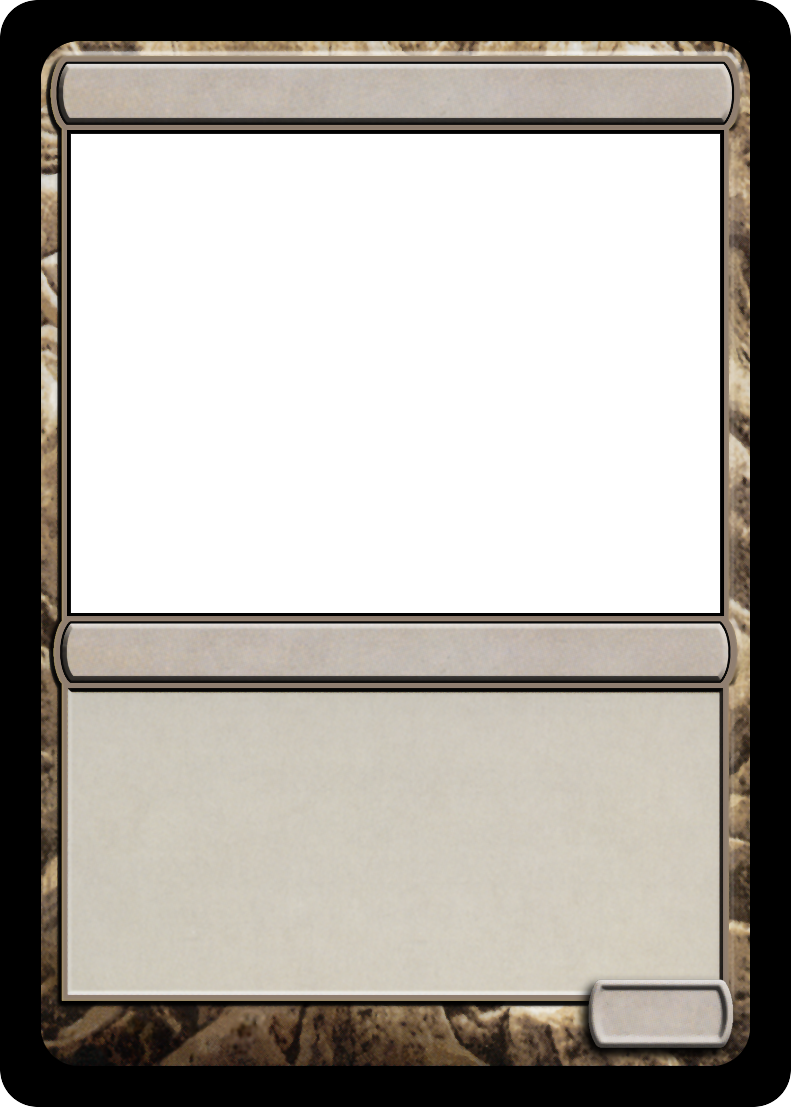
\includegraphics[width=\cardwidth cm, height=\cardheight cm]{fonds/fond_personnage.png}};

    %Titre
	\node[anchor=center] at (\titleX,\titleY) {\titlefont Assistante de Direction};

	%Image
	\node[anchor=center] at (\imageX,\imageY) {
\includegraphics[width=\imageWidth px, height=\imageHeight px]{images/P9_assistante.jpg}};
	\node[anchor=center] at (6.1,4.5) {
\includegraphics[width=12 px, height=6 px]{fonds2/legacy.jpg}};

	%Type
	\node[anchor=center] at (\typeX,\typeY) {\typefont Personnage};

	%Description
	\node[anchor=north west, text width=5.6cm] (description) at (\descriptionX,\descriptionY) {\descriptionfont\setsize{8}(Bonus) Au début de son tour, si l'assistante est assise a côté du manager, elle se défausse immédiatement de deux cartes.\par};

	%Punchline
	\node[anchor=north west, text width=5.6cm, below = 1pt of description] (punchline) {\punchlinefont\setsize{7}(Permanent) ``Il est très occupé. Le déjeuner du COPIL précède le cocktail du CODIR"\par};

	%Separateur !!!!!PAS TOUCHE!!!!!
	\fill[black,path fading=west] (description.south west) rectangle (punchline.north);
	\fill[black,path fading=east] (punchline.north) rectangle (description.south east);

	%Numéro !!!!!PAS TOUCHE!!!!!
	\node[anchor=center] at (\numberX,\numberY) {\numberfont 9/9};
\end{tikzpicture}\versoperso %Verso

%--------------------------CARTES SPECIALES------------------------------------------------------------------------------------------------ ANSSI
\begin{tikzpicture} %Recto
	%Fond
    \node[anchor=south west,inner sep=0] (carte) at (0,0) {
\includegraphics[width=7.1 cm, height=9.6 cm]{fonds/noir.png}};
    \node[anchor=center] at (carte.center) {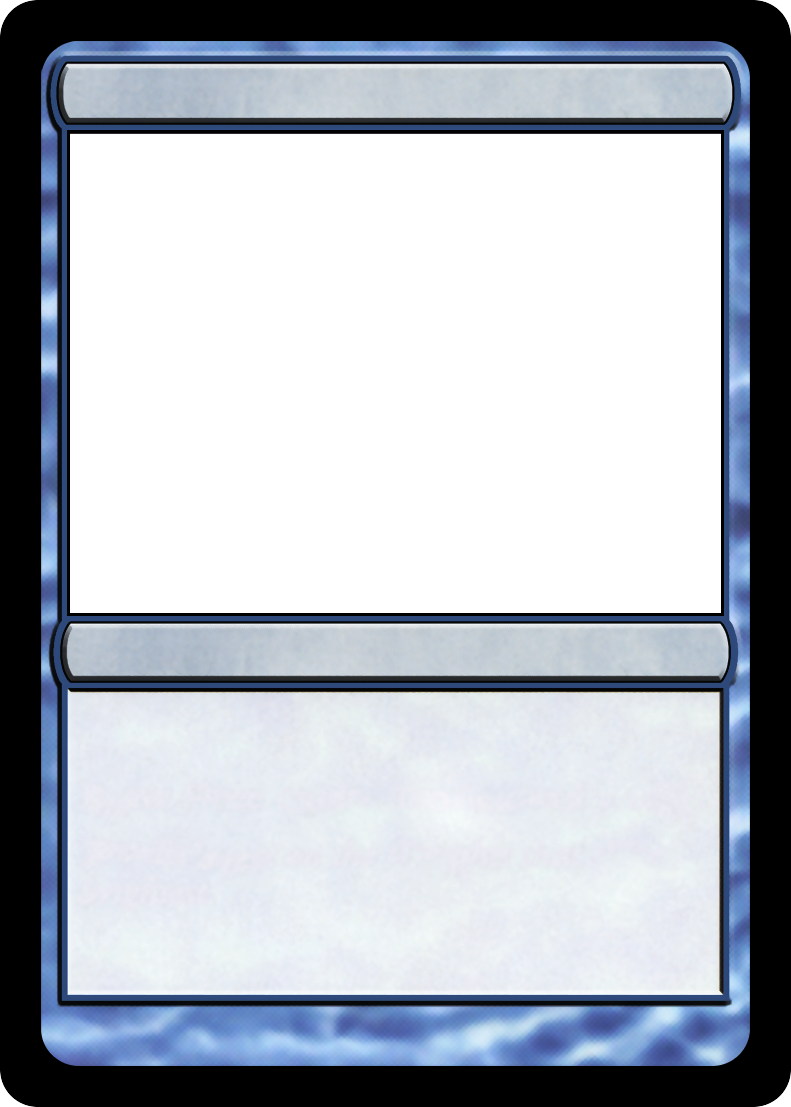
\includegraphics[width=\cardwidth cm, height=\cardheight cm]{fonds/fond_anssi.png}};

    %Titre
	\node[anchor=center] at (\titleX,\titleY) {\titlefont ANSSI};

	%Image
	\node[anchor=center] at (\imageX,\imageY) {
\includegraphics[width=\imageWidth px, height=\imageHeight px]{images/48_ANSSI.png}};
	\node[anchor=center] at (6.1,4.5) {
\includegraphics[width=12 px, height=6 px]{fonds2/legacy.jpg}};

	%Type
	\node[anchor=center] at (\typeX,\typeY) {\typefont Spécial (Permanent)};

	%Description
	\node[anchor=north west, text width=5.6cm] (description) at (\descriptionX,\descriptionY) {\descriptionfont\setsize{6} Placez cette carte devant vous seulement si vous êtes cryptologue. A chaque tour que vous débutez, révélez une carte, si vous ne commetez pas d'impair (la carte est paire) faites pivoter l'ANSSI d'un quart de tour (sens horaire). Après une rotation complète vous gagnez la partie.\par};

	%Punchline
	\node[anchor=north west, text width=5.6cm, below = 1pt of description] (punchline) {\punchlinefont\setsize{6} Convoitée par tous les joueurs, ne rêvez pas, à  moins de tricher, vous ne l'atteindrez  jamais.\par};

	%Separateur !!!!!PAS TOUCHE!!!!!
	\fill[black,path fading=west] (description.south west) rectangle (punchline.north);
	\fill[black,path fading=east] (punchline.north) rectangle (description.south east);
\end{tikzpicture}\verso %Verso


%--------------------------CARTES BONUS-------------------------------------------------------------------------------------------------
%!TEX root = lot1.tex
%--------------------------CARTES BONUS-------------------------------------------------------------------------------------------------
\begin{tikzpicture} %Recto
	%Fond
    \node[anchor=south west,inner sep=0] (carte) at (0,0) {
\includegraphics[width=7.1 cm, height=9.6 cm]{fonds/noir.png}};
    \node[anchor=center] at (carte.center) {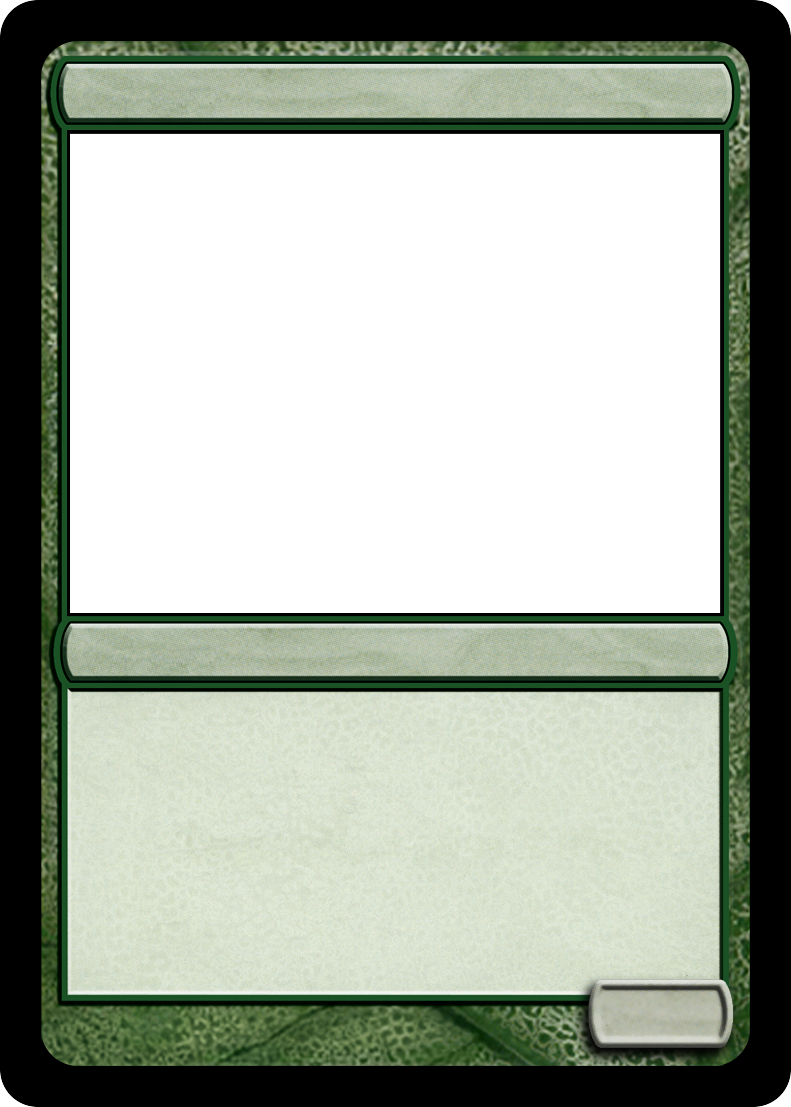
\includegraphics[width=\cardwidth cm, height=\cardheight cm]{fonds/fond_bonus.png}};

    %Titre
	\node[anchor=center] at (\titleX,\titleY) {\titlefont Absence enfant malade};

	%Image
	\node[anchor=center] at (\imageX,\imageY) {
\includegraphics[width=\imageWidth px, height=\imageHeight px]{images/UO_1_enfantmalade.jpg}};
	\node[anchor=center] at (6.1,4.5) {
\includegraphics[width=12 px, height=6 px]{fonds2/legacy.jpg}};

	%Type
	\node[anchor=center] at (\typeX,\typeY) {\typefont Bonus};

	%Description
	\node[anchor=north west, text width=5.6cm] (description) at (\descriptionX,\descriptionY) {\descriptionfont\setsize{8}Lorsqu’un joueur impute une carte malus contre vous, vous pouvez choisir d'utiliser immédiatement cette carte afin que le malus s’applique à un troisième joueur choisi par le manager.\par};


	%Numéro !!!!!PAS TOUCHE!!!!!
	\node[anchor=center] at (\numberX,\numberY) {\numberfont \cardnumber};
\end{tikzpicture}\verso %Verso

\begin{tikzpicture} %Recto
	%Fond
    \node[anchor=south west,inner sep=0] (carte) at (0,0) {\includegraphics[width=7.1 cm, height=9.6 cm]{fonds/noir.png}};
    \node[anchor=center] at (carte.center) {\includegraphics[width=\cardwidth cm, height=\cardheight cm]{fonds/fond_bonus.png}};

    %Titre
	\node[anchor=center] at (\titleX,\titleY) {\titlefont Vol business Paris New-York};

	%Image
	\node[anchor=center] at (\imageX,\imageY) {\includegraphics[width=\imageWidth px, height=\imageHeight px]{images/UO_2_vol.jpg}};
	\node[anchor=center] at (6.1,4.5) {\includegraphics[width=12 px, height=6 px]{fonds2/legacy.jpg}};

	%Type
	\node[anchor=center] at (\typeX,\typeY) {\typefont Bonus};

	%Description
	\node[anchor=north west, text width=5.6cm] (description) at (\descriptionX,\descriptionY) {\descriptionfont\setsize{8}Défaussez une carte. Les autres joueurs piochent une carte.\par};

	%Punchline
	\node[anchor=north west, text width=5.6cm, below = 1pt of description] (punchline) {\punchlinefont\setsize{8}``Vous avez consommé tout le budget conférence de vos collègues. Le confort du voyage compense largement leur mépris à votre égard.''\par};

	%Separateur !!!!!PAS TOUCHE!!!!!
	\fill[black,path fading=west] (description.south west) rectangle (punchline.north);
	\fill[black,path fading=east] (punchline.north) rectangle (description.south east);

	%Numéro !!!!!PAS TOUCHE!!!!!
	\node[anchor=center] at (\numberX,\numberY) {\numberfont \cardnumber};
\end{tikzpicture}\verso %Verso

\begin{tikzpicture} %Recto
	%Fond
    \node[anchor=south west,inner sep=0] (carte) at (0,0) {\includegraphics[width=7.1 cm, height=9.6 cm]{fonds/noir.png}};
    \node[anchor=center] at (carte.center) {\includegraphics[width=\cardwidth cm, height=\cardheight cm]{fonds/fond_bonus.png}};

    %Titre
	\node[anchor=center] at (\titleX,\titleY) {\titlefont Départ en conférence};

	%Image
	\node[anchor=center] at (\imageX,\imageY) {\includegraphics[width=\imageWidth px, height=\imageHeight px]{images/UO_3_Conference.jpg}};
	\node[anchor=center] at (6.1,4.5) {\includegraphics[width=12 px, height=6 px]{fonds2/legacy.jpg}};

	%Type
	\node[anchor=center] at (\typeX,\typeY) {\typefont Bonus};

	%Description
	\node[anchor=north west, text width=5.6cm] (description) at (\descriptionX,\descriptionY) {\descriptionfont\setsize{8}Défaussez une carte.\par};

	%Punchline
	\node[anchor=north west, text width=5.6cm, below = 1pt of description] (punchline) {\punchlinefont\setsize{8}Vous présentez un article appliqué à Crypto ! ``Unifying Leakage Models on a Rényi Day''.\par};

	%Separateur !!!!!PAS TOUCHE!!!!!
	\fill[black,path fading=west] (description.south west) rectangle (punchline.north);
	\fill[black,path fading=east] (punchline.north) rectangle (description.south east);

	%Numéro !!!!!PAS TOUCHE!!!!!
	\node[anchor=center] at (\numberX,\numberY) {\numberfont \cardnumber};
\end{tikzpicture}\verso %Verso

\begin{tikzpicture} %Recto
	%Fond
    \node[anchor=south west,inner sep=0] (carte) at (0,0) {\includegraphics[width=7.1 cm, height=9.6 cm]{fonds/noir.png}};
    \node[anchor=center] at (carte.center) {\includegraphics[width=\cardwidth cm, height=\cardheight cm]{fonds/fond_bonus.png}};

    %Titre
	\node[anchor=center] at (\titleX,\titleY) {\titlefont Organisation des conférences};

	%Image
	\node[anchor=center] at (\imageX,\imageY) {\includegraphics[width=\imageWidth px, height=\imageHeight px]{images/UO_4_orgaconf.jpg}};
	\node[anchor=center] at (6.1,4.5) {\includegraphics[width=12 px, height=6 px]{fonds2/legacy.jpg}};

	%Type
	\node[anchor=center] at (\typeX,\typeY) {\typefont Bonus (Interruption)};

	%Description
	\node[anchor=north west, text width=5.6cm] (description) at (\descriptionX,\descriptionY) {\descriptionfont\setsize{6}Lorsqu’un joueur joue une carte départ en conférence ou vol business, vous partez à sa place (vous défaussez à sa place). Vous pouvez aussi être fair et simplement l’imputer sans priver un de vos camarades, parce qu’au fond, vous êtes un gars bien.\par};

	%Punchline
	\node[anchor=north west, text width=5.6cm, below = 1pt of description] (punchline) {\punchlinefont\setsize{8}``Un grand pouvoir implique de grandes responsabilités.''\par};

	%Separateur !!!!!PAS TOUCHE!!!!!
	\fill[black,path fading=west] (description.south west) rectangle (punchline.north);
	\fill[black,path fading=east] (punchline.north) rectangle (description.south east);

	%Numéro !!!!!PAS TOUCHE!!!!!
	\node[anchor=center] at (\numberX,\numberY) {\numberfont \cardnumber};
\end{tikzpicture}\verso %Verso

\begin{tikzpicture} %Recto
	%Fond
    \node[anchor=south west,inner sep=0] (carte) at (0,0) {\includegraphics[width=7.1 cm, height=9.6 cm]{fonds/noir.png}};
    \node[anchor=center] at (carte.center) {\includegraphics[width=\cardwidth cm, height=\cardheight cm]{fonds/fond_bonus.png}};

    %Titre
	\node[anchor=center] at (\titleX,\titleY) {\titlefont Congés payés};

	%Image
	\node[anchor=center] at (\imageX,\imageY) {\includegraphics[width=\imageWidth px, height=\imageHeight px]{images/UO_5_Congés.jpg}};
	\node[anchor=center] at (6.1,4.5) {\includegraphics[width=12 px, height=6 px]{fonds2/legacy.jpg}};

	%Type
	\node[anchor=center] at (\typeX,\typeY) {\typefont Bonus};

	%Description
	\node[anchor=north west, text width=5.6cm] (description) at (\descriptionX,\descriptionY) {\descriptionfont\setsize{8}Vous pouvez défausser une carte supplémentaire et aller bronzer pendant que les autres travaillent à votre place.\par};

	%Punchline
	\node[anchor=north west, text width=5.6cm, below = 1pt of description] (punchline) {\punchlinefont\setsize{8}``923040 ACP est la seule ligne ERP qui vous satisfasse.''\par};

	%Separateur !!!!!PAS TOUCHE!!!!!
	\fill[black,path fading=west] (description.south west) rectangle (punchline.north);
	\fill[black,path fading=east] (punchline.north) rectangle (description.south east);

	%Numéro !!!!!PAS TOUCHE!!!!!
	\node[anchor=center] at (\numberX,\numberY) {\numberfont \cardnumber};
\end{tikzpicture}\verso %Verso

\begin{tikzpicture} %Recto
	%Fond
    \node[anchor=south west,inner sep=0] (carte) at (0,0) {\includegraphics[width=7.1 cm, height=9.6 cm]{fonds/noir.png}};
    \node[anchor=center] at (carte.center) {\includegraphics[width=\cardwidth cm, height=\cardheight cm]{fonds/fond_bonus.png}};

    %Titre
	\node[anchor=center] at (\titleX,\titleY) {\titlefont Crème br\^{u}lée du jeudi};

	%Image
	\node[anchor=center] at (\imageX,\imageY) {\includegraphics[width=\imageWidth px, height=\imageHeight px]{images/UO_6_Cremebrulee.jpg}};
	\node[anchor=center] at (6.1,4.5) {\includegraphics[width=12 px, height=6 px]{fonds2/legacy.jpg}};

	%Type
	\node[anchor=center] at (\typeX,\typeY) {\typefont Bonus };

	%Description
	\node[anchor=north west, text width=5.6cm] (description) at (\descriptionX,\descriptionY) {\descriptionfont\setsize{8}Défaussez une carte. Si vous avez fait une thèse en MPC, défaussez-en une deuxième.\par};

	%Punchline
	\node[anchor=north west, text width=5.6cm, below = 1pt of description] (punchline) {\punchlinefont\setsize{8}``Le saviez-vous ? Les contenants carrés ont un volume supérieur !''\par};

	%Separateur !!!!!PAS TOUCHE!!!!!
	\fill[black,path fading=west] (description.south west) rectangle (punchline.north);
	\fill[black,path fading=east] (punchline.north) rectangle (description.south east);

	%Numéro !!!!!PAS TOUCHE!!!!!
	\node[anchor=center] at (\numberX,\numberY) {\numberfont \cardnumber};
\end{tikzpicture}\verso %Verso

\begin{tikzpicture} %Recto
	%Fond
    \node[anchor=south west,inner sep=0] (carte) at (0,0) {\includegraphics[width=7.1 cm, height=9.6 cm]{fonds/noir.png}};
    \node[anchor=center] at (carte.center) {\includegraphics[width=\cardwidth cm, height=\cardheight cm]{fonds/fond_bonus.png}};

    %Titre
	\node[anchor=center] at (\titleX,\titleY) {\titlefont Demande KiSS validée !};

	%Image
	\node[anchor=center] at (\imageX,\imageY) {\includegraphics[width=\imageWidth px, height=\imageHeight px]{images/UO_7_KISSOK.jpg}};
	\node[anchor=center] at (6.1,4.5) {\includegraphics[width=12 px, height=6 px]{fonds2/legacy.jpg}};

	%Type
	\node[anchor=center] at (\typeX,\typeY) {\typefont Bonus};

	%Description
	\node[anchor=north west, text width=5.6cm] (description) at (\descriptionX,\descriptionY) {\descriptionfont\setsize{8}Les dieux sont de votre côté ! Votre demande KiSS à DSI vieille de deux ans vient d'être validée. Défaussez une carte.\par};

	%Punchline
	\node[anchor=north west, text width=5.6cm, below = 1pt of description] (punchline) {\punchlinefont\setsize{8}``Mais est-ce que votre demande de demande KiSS a bien été validée ?''\par};

	%Separateur !!!!!PAS TOUCHE!!!!!
	\fill[black,path fading=west] (description.south west) rectangle (punchline.north);
	\fill[black,path fading=east] (punchline.north) rectangle (description.south east);

	%Numéro !!!!!PAS TOUCHE!!!!!
	\node[anchor=center] at (\numberX,\numberY) {\numberfont \cardnumber};
\end{tikzpicture}\verso %Verso

\begin{tikzpicture} %Recto
	%Fond
    \node[anchor=south west,inner sep=0] (carte) at (0,0) {\includegraphics[width=7.1 cm, height=9.6 cm]{fonds/noir.png}};
    \node[anchor=center] at (carte.center) {\includegraphics[width=\cardwidth cm, height=\cardheight cm]{fonds/fond_bonus.png}};

    %Titre
	\node[anchor=center] at (\titleX,\titleY) {\titlefont Cloud Manager !};

	%Image
	\node[anchor=center] at (\imageX,\imageY) {\includegraphics[width=\imageWidth px, height=\imageHeight px]{images/UO_8_Cloudmanager.jpg}};
	\node[anchor=center] at (6.1,4.5) {\includegraphics[width=12 px, height=6 px]{fonds2/legacy.jpg}};

	%Type
	\node[anchor=center] at (\typeX,\typeY) {\typefont Bonus (Interruption)};

	%Description
	\node[anchor=north west, text width=5.6cm] (description) at (\descriptionX,\descriptionY) {\descriptionfont\setsize{7}Vous attendez de votre équipe une certaine autonomie. Lorsque vous devez piocher une carte, défaussez celle-ci et demandez à un autre joueur de piocher à votre place.\par};

	%Punchline
	\node[anchor=north west, text width=5.6cm, below = 1pt of description] (punchline) {\punchlinefont\setsize{7}``Tu es vraiment le meilleur pour ce type de tâche. Il vaut mieux que tu le fasses. Je te fais parfaitement confiance.''\par};

	%Separateur !!!!!PAS TOUCHE!!!!!
	\fill[black,path fading=west] (description.south west) rectangle (punchline.north);
	\fill[black,path fading=east] (punchline.north) rectangle (description.south east);

	%Numéro !!!!!PAS TOUCHE!!!!!
	\node[anchor=center] at (\numberX,\numberY) {\numberfont \cardnumber};
\end{tikzpicture}\verso %Verso

\begin{tikzpicture} %Recto
	%Fond
    \node[anchor=south west,inner sep=0] (carte) at (0,0) {\includegraphics[width=7.1 cm, height=9.6 cm]{fonds/noir.png}};
    \node[anchor=center] at (carte.center) {\includegraphics[width=\cardwidth cm, height=\cardheight cm]{fonds/fond_bonus.png}};

    %Titre
	\node[anchor=center] at (\titleX,\titleY) {\titlefont Obeya};

	%Image
	\node[anchor=center] at (\imageX,\imageY) {\includegraphics[width=\imageWidth px, height=\imageHeight px]{images/UO_9_Obeya.jpg}};
	\node[anchor=center] at (6.1,4.5) {\includegraphics[width=12 px, height=6 px]{fonds2/legacy.jpg}};

	%Type
	\node[anchor=center] at (\typeX,\typeY) {\typefont Bonus 	};

	%Description
	\node[anchor=north west, text width=5.6cm] (description) at (\descriptionX,\descriptionY) {\descriptionfont\setsize{8}Vous et le cryptologue (doit être présent et autre que vous), faisant habilement semblant de travailler, vous défaussez une carte de votre choix.\par};

	%Punchline
	\node[anchor=north west, text width=5.6cm, below = 1pt of description] (punchline) {\punchlinefont\setsize{8}``Tiens ! Ils ont élevé les tables.''\par};

	%Separateur !!!!!PAS TOUCHE!!!!!
	\fill[black,path fading=west] (description.south west) rectangle (punchline.north);
	\fill[black,path fading=east] (punchline.north) rectangle (description.south east);

	%Numéro !!!!!PAS TOUCHE!!!!!
	\node[anchor=center] at (\numberX,\numberY) {\numberfont \cardnumber};
\end{tikzpicture}\verso %Verso

\begin{tikzpicture} %Recto
	%Fond
    \node[anchor=south west,inner sep=0] (carte) at (0,0) {\includegraphics[width=7.1 cm, height=9.6 cm]{fonds/noir.png}};
    \node[anchor=center] at (carte.center) {\includegraphics[width=\cardwidth cm, height=\cardheight cm]{fonds/fond_bonus.png}};

    %Titre
	\node[anchor=center] at (\titleX,\titleY) {\titlefont Habilitation SD};

	%Image
	\node[anchor=center] at (\imageX,\imageY) {\includegraphics[width=\imageWidth px, height=\imageHeight px]{images/UO_10_habilitation.jpg}};
	\node[anchor=center] at (6.1,4.5) {\includegraphics[width=12 px, height=6 px]{fonds2/legacy.jpg}};

	%Type
	\node[anchor=center] at (\typeX,\typeY) {\typefont Bonus (Permanent)};

	%Description
	\node[anchor=north west, text width=5.6cm] (description) at (\descriptionX,\descriptionY) {\descriptionfont\setsize{6}Posez cette carte devant vous en demande. Au début de votre tour, révélez une carte. L'habilitation devient validée si la valeur est paire (seulement si elle vaut 8 si vous êtes Julien). Tant que vous êtes habilité, vous pouvez défausser une carte à la fin de votre tour. \par};

	%Punchline
	\node[anchor=north west, text width=5.6cm, below = 1pt of description] (punchline) {\punchlinefont\setsize{8}``Permet l'ouverture de la zone SD.''\par};

	%Separateur !!!!!PAS TOUCHE!!!!!
	\fill[black,path fading=west] (description.south west) rectangle (punchline.north);
	\fill[black,path fading=east] (punchline.north) rectangle (description.south east);

	%Numéro !!!!!PAS TOUCHE!!!!!
	\node[anchor=center] at (\numberX,\numberY) {\numberfont \cardnumber};
\end{tikzpicture}\verso %Verso

\begin{tikzpicture} %Recto
	%Fond
    \node[anchor=south west,inner sep=0] (carte) at (0,0) {\includegraphics[width=7.1 cm, height=9.6 cm]{fonds/noir.png}};
    \node[anchor=center] at (carte.center) {\includegraphics[width=\cardwidth cm, height=\cardheight cm]{fonds/fond_bonus.png}};

    %Titre
	\node[anchor=center] at (\titleX,\titleY) {\titlefont Habilitation SD};

	%Image
	\node[anchor=center] at (\imageX,\imageY) {\includegraphics[width=\imageWidth px, height=\imageHeight px]{images/UO_11_habilitation.jpg}};
	\node[anchor=center] at (6.1,4.5) {\includegraphics[width=12 px, height=6 px]{fonds2/legacy.jpg}};

	%Type
	\node[anchor=center] at (\typeX,\typeY) {\typefont Bonus (Permanent)};

	%Description
	\node[anchor=north west, text width=5.6cm] (description) at (\descriptionX,\descriptionY) {\descriptionfont\setsize{6}Posez cette carte devant vous en demande. Au début de votre tour, révélez une carte. L'habilitation devient validée si la valeur est paire (seulement si elle vaut 8 si vous êtes Julien). Tant que vous êtes habilité, vous pouvez défausser une carte à la fin de votre tour.\par};

	%Punchline
	\node[anchor=north west, text width=5.6cm, below = 1pt of description] (punchline) {\punchlinefont\setsize{8}``Permet l'ouverture de la zone SD.''\par};

	%Separateur !!!!!PAS TOUCHE!!!!!
	\fill[black,path fading=west] (description.south west) rectangle (punchline.north);
	\fill[black,path fading=east] (punchline.north) rectangle (description.south east);

	%Numéro !!!!!PAS TOUCHE!!!!!
	\node[anchor=center] at (\numberX,\numberY) {\numberfont \cardnumber};
\end{tikzpicture}\verso %Verso


\begin{tikzpicture} %Recto
	%Fond
    \node[anchor=south west,inner sep=0] (carte) at (0,0) {\includegraphics[width=7.1 cm, height=9.6 cm]{fonds/noir.png}};
    \node[anchor=center] at (carte.center) {\includegraphics[width=\cardwidth cm, height=\cardheight cm]{fonds/fond_bonus.png}};

    %Titre
	\node[anchor=center] at (\titleX,\titleY) {\titlefont Coffre CD (Permanent)};

	%Image
	\node[anchor=center] at (\imageX,\imageY) {\includegraphics[width=\imageWidth px, height=\imageHeight px]{images/UO_12_coffre.jpg}};
	\node[anchor=center] at (6.1,4.5) {\includegraphics[width=12 px, height=6 px]{fonds2/legacy.jpg}};

	%Type
	\node[anchor=center] at (\typeX,\typeY) {\typefont Bonus (Permanent)};

	%Description
	\node[anchor=north west, text width=5.6cm] (description) at (\descriptionX,\descriptionY) {\descriptionfont\setsize{7}Posez cette carte devant vous en demande. Vous pouvez y ranger vos documents CD, un saucisson, mais également une carte que vous placez dessous. Vous pouvez échanger une carte du coffre SD et de votre main au début de votre tour.\par};

	%Punchline
	\node[anchor=north west, text width=5.6cm, below = 1pt of description] (punchline) {\punchlinefont\setsize{8}``N'oubliez pas la combinaison.''\par};

	%Separateur !!!!!PAS TOUCHE!!!!!
	\fill[black,path fading=west] (description.south west) rectangle (punchline.north);
	\fill[black,path fading=east] (punchline.north) rectangle (description.south east);

	%Numéro !!!!!PAS TOUCHE!!!!!
	\node[anchor=center] at (\numberX,\numberY) {\numberfont \cardnumber};
\end{tikzpicture}\verso %Verso

\begin{tikzpicture} %Recto
	%Fond
    \node[anchor=south west,inner sep=0] (carte) at (0,0) {\includegraphics[width=7.1 cm, height=9.6 cm]{fonds/noir.png}};
    \node[anchor=center] at (carte.center) {\includegraphics[width=\cardwidth cm, height=\cardheight cm]{fonds/fond_bonus.png}};

    %Titre
	\node[anchor=center] at (\titleX,\titleY) {\titlefont Serveur Pirate Calcul};

	%Image
	\node[anchor=center] at (\imageX,\imageY) {\includegraphics[width=\imageWidth px, height=\imageHeight px]{images/UO_13_Serveur.jpg}};
	\node[anchor=center] at (6.1,4.5) {\includegraphics[width=12 px, height=6 px]{fonds2/legacy.jpg}};

	%Type
	\node[anchor=center] at (\typeX,\typeY) {\typefont Bonus (Permanent)};

	%Description
	\node[anchor=north west, text width=5.6cm] (description) at (\descriptionX,\descriptionY) {\descriptionfont\setsize{8}Posez cette carte devant vous. Tant que vous avez le serveur pirate devant vous, l'effet de paralysie du personnage DSI est ignoré s'il tombe sur vous.\par};

	%Punchline
	\node[anchor=north west, text width=5.6cm, below = 1pt of description] (punchline) {\punchlinefont\setsize{8}``ssh -X julien@calcul.''\par};

	%Separateur !!!!!PAS TOUCHE!!!!!
	\fill[black,path fading=west] (description.south west) rectangle (punchline.north);
	\fill[black,path fading=east] (punchline.north) rectangle (description.south east);

	%Numéro !!!!!PAS TOUCHE!!!!!
	\node[anchor=center] at (\numberX,\numberY) {\numberfont \cardnumber};
\end{tikzpicture}\verso %Verso




\begin{tikzpicture} %Recto
	%Fond
    \node[anchor=south west,inner sep=0] (carte) at (0,0) {\includegraphics[width=7.1 cm, height=9.6 cm]{fonds/noir.png}};
    \node[anchor=center] at (carte.center) {\includegraphics[width=\cardwidth cm, height=\cardheight cm]{fonds/fond_bonus.png}};

    %Titre
	\node[anchor=center] at (\titleX,\titleY) {\titlefont Grève !! Télétravail et vélo};

	%Image
	\node[anchor=center] at (\imageX,\imageY) {\includegraphics[width=\imageWidth px, height=\imageHeight px]{images/UO_14_velogreve.jpg}};
	\node[anchor=center] at (6.1,4.5) {\includegraphics[width=12 px, height=6 px]{fonds2/legacy.jpg}};

	%Type
	\node[anchor=center] at (\typeX,\typeY) {\typefont Bonus };

	%Description
	\node[anchor=north west, text width=5.6cm] (description) at (\descriptionX,\descriptionY) {\descriptionfont\setsize{8}Chaque joueur fait le tour de la table puis s'assied une place plus loin. Sauf vous qui êtes en télétravail et défaussez une carte.\par};

	%Punchline
	\node[anchor=north west, text width=5.6cm, below = 1pt of description] (punchline) {\punchlinefont\setsize{8}``Allumez votre communicator avant de lancer Game of Thrones.''\par};

	%Separateur !!!!!PAS TOUCHE!!!!!
	\fill[black,path fading=west] (description.south west) rectangle (punchline.north);
	\fill[black,path fading=east] (punchline.north) rectangle (description.south east);

	%Numéro !!!!!PAS TOUCHE!!!!!
	\node[anchor=center] at (\numberX,\numberY) {\numberfont \cardnumber};
\end{tikzpicture}\verso %Verso





\begin{tikzpicture} %Recto
	%Fond
    \node[anchor=south west,inner sep=0] (carte) at (0,0) {\includegraphics[width=7.1 cm, height=9.6 cm]{fonds/noir.png}};
    \node[anchor=center] at (carte.center) {\includegraphics[width=\cardwidth cm, height=\cardheight cm]{fonds/fond_bonus.png}};

    %Titre
	\node[anchor=center] at (\titleX,\titleY) {\titlefont Laurent NiceBro'};

	%Image
	\node[anchor=center] at (\imageX,\imageY) {\includegraphics[width=\imageWidth px, height=\imageHeight px]{images/UO_15_LaurentNiceBro.png}};
	\node[anchor=center] at (6.1,4.5) {\includegraphics[width=12 px, height=6 px]{fonds2/legacy.jpg}};

	%Type
	\node[anchor=center] at (\typeX,\typeY) {\typefont Bonus };

	%Description
	\node[anchor=north west, text width=5.6cm] (description) at (\descriptionX,\descriptionY) {\descriptionfont\setsize{8}Un manager développeur vous donne un coup de main pour développer une librairie crypto aux interfaces petit poney. Défaussez une carte.\par};

	%Punchline
	\node[anchor=north west, text width=5.6cm, below = 1pt of description] (punchline) {\punchlinefont\setsize{8}``Chemise blanche aussi impeccable que les APIs. C'est le secret.''\par};

	%Separateur !!!!!PAS TOUCHE!!!!!
	\fill[black,path fading=west] (description.south west) rectangle (punchline.north);
	\fill[black,path fading=east] (punchline.north) rectangle (description.south east);

	%Numéro !!!!!PAS TOUCHE!!!!!
	\node[anchor=center] at (\numberX,\numberY) {\numberfont \cardnumber};
\end{tikzpicture}\verso %Verso


\begin{tikzpicture} %Recto
	%Fond
    \node[anchor=south west,inner sep=0] (carte) at (0,0) {\includegraphics[width=7.1 cm, height=9.6 cm]{fonds/noir.png}};
    \node[anchor=center] at (carte.center) {\includegraphics[width=\cardwidth cm, height=\cardheight cm]{fonds/fond_bonus.png}};

    %Titre
	\node[anchor=center] at (\titleX,\titleY) {\titlefont Résilience au mal};

	%Image
	\node[anchor=center] at (\imageX,\imageY) {\includegraphics[width=\imageWidth px, height=\imageHeight px]{images/UO_16_resistance.jpg}};
	\node[anchor=center] at (6.1,4.5) {\includegraphics[width=12 px, height=6 px]{fonds2/legacy.jpg}};

	%Type
	\node[anchor=center] at (\typeX,\typeY) {\typefont Bonus(Interruption)};

	%Description
	\node[anchor=north west, text width=5.6cm] (description) at (\descriptionX,\descriptionY) {\descriptionfont\setsize{8}Utilisez cette carte pour annuler un effet MALUS ou détruire un permanent MALUS de votre choix.\par};

	%Punchline
	\node[anchor=north west, text width=5.6cm, below = 1pt of description] (punchline) {\punchlinefont\setsize{8}``Process, DSI, collègue toxique, tel un paladin rien ne peut vous arrêter.''\par};

	%Separateur !!!!!PAS TOUCHE!!!!!
	\fill[black,path fading=west] (description.south west) rectangle (punchline.north);
	\fill[black,path fading=east] (punchline.north) rectangle (description.south east);

	%Numéro !!!!!PAS TOUCHE!!!!!
	\node[anchor=center] at (\numberX,\numberY) {\numberfont \cardnumber};
\end{tikzpicture}\verso %Verso


\begin{tikzpicture} %Recto
	%Fond
    \node[anchor=south west,inner sep=0] (carte) at (0,0) {\includegraphics[width=7.1 cm, height=9.6 cm]{fonds/noir.png}};
    \node[anchor=center] at (carte.center) {\includegraphics[width=\cardwidth cm, height=\cardheight cm]{fonds/fond_bonus.png}};

    %Titre
	\node[anchor=center] at (\titleX,\titleY) {\titlefont Dream Team};

	%Image
	\node[anchor=center] at (\imageX,\imageY) {\includegraphics[width=\imageWidth px, height=\imageHeight px]{images/UO_17_Dreamteam.jpg}};
	\node[anchor=center] at (6.1,4.5) {\includegraphics[width=12 px, height=6 px]{fonds2/legacy.jpg}};

	%Type
	\node[anchor=center] at (\typeX,\typeY) {\typefont Bonus };

	%Description
	\node[anchor=north west, text width=5.6cm] (description) at (\descriptionX,\descriptionY) {\descriptionfont\setsize{8}Vous faites partie de LCH. Il n'y a rien à ajouter. Vous méritez de gagner cette partie. Défaussez deux cartes.\par};

	%Punchline
	\node[anchor=north west, text width=5.6cm, below = 1pt of description] (punchline) {\punchlinefont\setsize{8}``Il faudrait être fou pour en partir !''\par};

	%Separateur !!!!!PAS TOUCHE!!!!!
	\fill[black,path fading=west] (description.south west) rectangle (punchline.north);
	\fill[black,path fading=east] (punchline.north) rectangle (description.south east);

	%Numéro !!!!!PAS TOUCHE!!!!!
	\node[anchor=center] at (\numberX,\numberY) {\numberfont \cardnumber};
\end{tikzpicture}\verso %Verso

%--------------------------CARTES SPECIFIQUES-------------------------------------------------------------------------------------------
%!TEX root = lot1.tex

%--------------------------CARTES DOUBLES-------------------------------------------------------------------------------------------------

\begin{tikzpicture} %Recto
	%Fond
    \node[anchor=south west,inner sep=0] (carte) at (0,0) {\includegraphics[width=7.1 cm, height=9.6 cm]{fonds/noir.png}};
    \node[anchor=center] at (carte.center) {\includegraphics[width=\cardwidth cm, height=\cardheight cm]{fonds/fond_hybride.png}};

    %Titre
	\node[anchor=center] at (\titleX,\titleY) {\titlefont SRR};

	%Image
	\node[anchor=center] at (\imageX,\imageY) {\includegraphics[width=\imageWidth px, height=\imageHeight px]{images/UO_18_VDD.jpg}};
	\node[anchor=center] at (6.1,4.5) {\includegraphics[width=12 px, height=6 px]{fonds2/legacy.jpg}};

	%Type
	\node[anchor=center] at (\typeX,\typeY) {\typefont Bonus - Malus};

	%Description bonus
	\node[anchor=north west, text width=5.6cm] (description1) at (\descriptionX,\descriptionY) {\descriptionfont\setsize{7}(Bonus) Presque aucun trou dans la raquette. Avouez qu'un cryptologue vous a aidé hein ? L'ingénieur système défausse une carte.\par};

	%Description malus
	\node[anchor=north west, text width=5.6cm, below = 1pt of description1] (description2) {\descriptionfont\setsize{7}(Malus) Jouez cette carte contre l'Ingénieur Système. Pas de versionnage, rien n'est cohérent. Vous vous foutez du monde, cela mérite bien de piocher une carte !\par};

	%Separateur !!!!!PAS TOUCHE!!!!!
	\fill[black,path fading=west] (description1.south west) rectangle (description2.north);
	\fill[black,path fading=east] (description2.north) rectangle (description1.south east);

	%Numéro !!!!!PAS TOUCHE!!!!!
	\node[anchor=center] at (\numberX,\numberY) {\numberfont \cardnumber};
\end{tikzpicture}\verso %Verso


\begin{tikzpicture} %Recto
	%Fond
    \node[anchor=south west,inner sep=0] (carte) at (0,0) {\includegraphics[width=7.1 cm, height=9.6 cm]{fonds/noir.png}};
    \node[anchor=center] at (carte.center) {\includegraphics[width=\cardwidth cm, height=\cardheight cm]{fonds/fond_hybride.png}};

    %Titre
	\node[anchor=center] at (\titleX,\titleY) {\titlefont My beloved HoD};

	%Image
	\node[anchor=center] at (\imageX,\imageY) {\includegraphics[width=\imageWidth px, height=\imageHeight px]{images/hod.jpg}};
	\node[anchor=center] at (6.1,4.5) {\includegraphics[width=12 px, height=6 px]{fonds2/legacy.jpg}};

	%Type
	\node[anchor=center] at (\typeX,\typeY) {\typefont Bonus - Malus};

	%Description bonus
	\node[anchor=north west, text width=5.6cm] (description1) at (\descriptionX,\descriptionY) {\descriptionfont\setsize{6}(Bonus) Votre équipe est dynamique, reconnue du client et de votre hiérarchie. Tout cela grâce à votre management éclairé, ou alors ils sont très autonomes, ce qui indique un sens aigû du recrutement. Même si votre génie vous fatigue, le manager défausse une carte.\par};

	%Description malus
	\node[anchor=north west, text width=5.6cm, below = 1pt of description1] (description2) {\descriptionfont\setsize{6}(Malus) Plan de charge inconsistant, EAA en retard à base de sauvages copiés/collés. Le manager pioche une carte.\par};
	%Punchline
	\node[anchor=north west, text width=5.6cm, below = 33pt of description] (punchline) {\punchlinefont\setsize{6}``- My name is Doe, Garry Doe.''\par};
	
	%Separateur !!!!!PAS TOUCHE!!!!!
	\fill[black,path fading=west] (description1.south west) rectangle (description2.north);
	\fill[black,path fading=east] (description2.north) rectangle (description1.south east);

	%Numéro !!!!!PAS TOUCHE!!!!!
	\node[anchor=center] at (\numberX,\numberY) {\numberfont \cardnumber};
\end{tikzpicture}\verso %Verso


\begin{tikzpicture} %Recto
	%Fond
    \node[anchor=south west,inner sep=0] (carte) at (0,0) {\includegraphics[width=7.1 cm, height=9.6 cm]{fonds/noir.png}};
    \node[anchor=center] at (carte.center) {\includegraphics[width=\cardwidth cm, height=\cardheight cm]{fonds/fond_hybride.png}};

    %Titre
	\node[anchor=center] at (\titleX,\titleY) {\titlefont STR (Software Test Review)};

	%Image
	\node[anchor=center] at (\imageX,\imageY) {\includegraphics[width=\imageWidth px, height=\imageHeight px]{images/developpement_code.jpg}};
	\node[anchor=center] at (6.1,4.5) {\includegraphics[width=12 px, height=6 px]{fonds2/legacy.jpg}};

	%Type
	\node[anchor=center] at (\typeX,\typeY) {\typefont Bonus - Malus};

	%Description bonus
	\node[anchor=north west, text width=5.6cm] (description1) at (\descriptionX,\descriptionY) {\descriptionfont\setsize{7}(Bonus) Vous êtes tellement bon qu'on devrait carrément skipper la phase d'IVQ. Le développeur pioche une carte.\par};
	%Description malus
	\node[anchor=north west, text width=5.6cm, below = 1pt of description1] (description2) {\descriptionfont\setsize{7}(Malus) Ca ne compile pas, c'est truffé de bug, vous travailliez sur autre chose en douce n'est-ce pas ? Piochez une carte pour la peine.\par};
	%Punchline
	\node[anchor=north west, text width=5.6cm, below = 29pt of description] (punchline) {\punchlinefont\setsize{7}``{  gcc *.c -o \$EXE -Wall -brainfuck}''\par};
	%Separateur !!!!!PAS TOUCHE!!!!!
	\fill[black,path fading=west] (description1.south west) rectangle (description2.north);
	\fill[black,path fading=east] (description2.north) rectangle (description1.south east);

	%Numéro !!!!!PAS TOUCHE!!!!!
	\node[anchor=center] at (\numberX,\numberY) {\numberfont \cardnumber};
\end{tikzpicture}\verso %Verso


\begin{tikzpicture} %Recto
	%Fond
    \node[anchor=south west,inner sep=0] (carte) at (0,0) {\includegraphics[width=7.1 cm, height=9.6 cm]{fonds/noir.png}};
    \node[anchor=center] at (carte.center) {\includegraphics[width=\cardwidth cm, height=\cardheight cm]{fonds/fond_hybride.png}};

    %Titre
	\node[anchor=center] at (\titleX,\titleY) {\titlefont Jeudi de la sécurité};

	%Image
	\node[anchor=center] at (\imageX,\imageY) {\includegraphics[width=\imageWidth px, height=\imageHeight px]{images/UO_22_marketing.jpg}};
	\node[anchor=center] at (6.1,4.5) {\includegraphics[width=12 px, height=6 px]{fonds2/legacy.jpg}};

	%Type
	\node[anchor=center] at (\typeX,\typeY) {\typefont Bonus - Malus};

	%Description bonus
	\node[anchor=north west, text width=5.6cm] (description1) at (\descriptionX,\descriptionY) {\descriptionfont\setsize{6}(Bonus) Le marketting défausse une carte pour une présentation presque sans approximations d'une thématique technique à laquelle il ne maîtrise rien.\par};
	%Description malus
	\node[anchor=north west, text width=5.6cm, below = 1pt of description1] (description2) {\descriptionfont\setsize{6}(Malus) Vous n'avez pas réalisé que vous êtes en train de faire la promotion d'une librairie de la concurrence. Cela mérite bien de piocher une carte et lire quelques articles Wikipedia.\par};
	%Punchline
	\node[anchor=north west, text width=5.6cm, below = 29pt of description] (punchline) {\punchlinefont\setsize{6}``Pour cette punchline, voir avec le marketting.''\par};
	%Separateur !!!!!PAS TOUCHE!!!!!
	\fill[black,path fading=west] (description1.south west) rectangle (description2.north);
	\fill[black,path fading=east] (description2.north) rectangle (description1.south east);

	%Numéro !!!!!PAS TOUCHE!!!!!
	\node[anchor=center] at (\numberX,\numberY) {\numberfont \cardnumber};
\end{tikzpicture}\verso %Verso

\begin{tikzpicture} %Recto
	%Fond
    \node[anchor=south west,inner sep=0] (carte) at (0,0) {\includegraphics[width=7.1 cm, height=9.6 cm]{fonds/noir.png}};
    \node[anchor=center] at (carte.center) {\includegraphics[width=\cardwidth cm, height=\cardheight cm]{fonds/fond_hybride.png}};

    %Titre
	\node[anchor=center] at (\titleX,\titleY) {\titlefont Proposition de thèse};

	%Image
	\node[anchor=center] at (\imageX,\imageY) {\includegraphics[width=\imageWidth px, height=\imageHeight px]{images/UO_23_stage.jpg}};
	\node[anchor=center] at (6.1,4.5) {\includegraphics[width=12 px, height=6 px]{fonds2/legacy.jpg}};

	%Type
	\node[anchor=center] at (\typeX,\typeY) {\typefont Bonus - Malus};

	%Description bonus
	\node[anchor=north west, text width=5.6cm] (description1) at (\descriptionX,\descriptionY) {\descriptionfont\setsize{7}(Bonus) Le stagiaire obtient automatiquement un CDI à ce tour (nouveau contrat).\par};
	%Description malus
	\node[anchor=north west, text width=5.6cm, below = 1pt of description1] (description2) {\descriptionfont\setsize{7}(Malus) Un CDI extérieur est proposé à ce petit ingrat de stagiaire qui accepte le poste ! Il ne peut y avoir de nouveau contrat à ce tour.\par};
	%Punchline
	\node[anchor=north west, text width=5.6cm, below = 27pt of description] (punchline) {\punchlinefont\setsize{7}``Je suis de la génération Y, je mérite bien plus que cette grille d'embauche.''\par};

	%Separateur !!!!!PAS TOUCHE!!!!!
	\fill[black,path fading=west] (description1.south west) rectangle (description2.north);
	\fill[black,path fading=east] (description2.north) rectangle (description1.south east);

	%Numéro !!!!!PAS TOUCHE!!!!!
	\node[anchor=center] at (\numberX,\numberY) {\numberfont \cardnumber};
\end{tikzpicture}\verso %Verso


\begin{tikzpicture} %Recto
	%Fond
    \node[anchor=south west,inner sep=0] (carte) at (0,0) {\includegraphics[width=7.1 cm, height=9.6 cm]{fonds/noir.png}};
    \node[anchor=center] at (carte.center) {\includegraphics[width=\cardwidth cm, height=\cardheight cm]{fonds/fond_hybride.png}};

    %Titre
	\node[anchor=center] at (\titleX,\titleY) {\titlefont Demande KiSS refusée !};

	%Image
	\node[anchor=center] at (\imageX,\imageY) {\includegraphics[width=\imageWidth px, height=\imageHeight px]{images/UO_24_kiss.jpg}};
	\node[anchor=center] at (6.1,4.5) {\includegraphics[width=12 px, height=6 px]{fonds2/legacy.jpg}};

	%Type
	\node[anchor=center] at (\typeX,\typeY) {\typefont Bonus - Malus};

	%Description bonus
	\node[anchor=north west, text width=5.6cm] (description1) at (\descriptionX,\descriptionY) {\descriptionfont\setsize{6}(Bonus) Gnark gnark gnark. Cela a beau être votre quotidien de DSI, ça vous fait toujours autant plaisir. Seul DSI peut jouer cette carte pour forcer un autre joueur à piocher.\par};
	%Description malus
	\node[anchor=north west, text width=5.6cm, below = 1pt of description1] (description2) {\descriptionfont\setsize{6}(Malus) Mais, mais, mais, non ! Cet utilisateur obstiné réémet sa demande pour la dixième fois. Ce surcroît de travail épuise le joueur DSI qui pioche une carte.\par};
	%Punchline
	\node[anchor=north west, text width=5.6cm, below = 27pt of description] (punchline) {\punchlinefont\setsize{6}``N'oubliez pas de remplir notre questionnaire de satisfaction.''\par};

	%Separateur !!!!!PAS TOUCHE!!!!!
	\fill[black,path fading=west] (description1.south west) rectangle (description2.north);
	\fill[black,path fading=east] (description2.north) rectangle (description1.south east);

	%Numéro !!!!!PAS TOUCHE!!!!!
	\node[anchor=center] at (\numberX,\numberY) {\numberfont \cardnumber};
\end{tikzpicture}\verso %Verso
%%%%%%%%%%%%%%%%%%%%%%%%%%%%%%%%%%%%%%%%%%%%%

\begin{tikzpicture} %Recto
	%Fond
    \node[anchor=south west,inner sep=0] (carte) at (0,0) {\includegraphics[width=7.1 cm, height=9.6 cm]{fonds/noir.png}};
    \node[anchor=center] at (carte.center) {\includegraphics[width=\cardwidth cm, height=\cardheight cm]{fonds/fond_hybride.png}};

    %Titre
	\node[anchor=center] at (\titleX,\titleY) {\titlefont Invention géniale};

	%Image
	\node[anchor=center] at (\imageX,\imageY) {\includegraphics[width=\imageWidth px, height=\imageHeight px]{images/invention.jpg}};
	\node[anchor=center] at (6.1,4.5) {\includegraphics[width=12 px, height=6 px]{fonds2/legacy.jpg}};

	%Type
	\node[anchor=center] at (\typeX,\typeY) {\typefont Bonus - Malus};

	%Description bonus
	\node[anchor=north west, text width=5.6cm] (description1) at (\descriptionX,\descriptionY) {\descriptionfont\setsize{7}(Bonus) Votre invention est clairement une opportunité majeure pour le groupe. Le cryptologue défausse une carte.\par};
	%Description malus
	\node[anchor=north west, text width=5.6cm, below = 1pt of description1] (description2) {\descriptionfont\setsize{7}(Malus) Bien sûr que c'est génial. Mais la priorité est de produire cette perforatrice de bande. Le cryptologue pioche une carte de désespoir.\par};
	%Punchline
	\node[anchor=north west, text width=5.6cm, below = 29pt of description] (punchline) {\punchlinefont\setsize{6}``THALES, innover aujourd'hui avec les technologies d'avant hier.''\par};

	%Separateur !!!!!PAS TOUCHE!!!!!
	\fill[black,path fading=west] (description1.south west) rectangle (description2.north);
	\fill[black,path fading=east] (description2.north) rectangle (description1.south east);

	%Numéro !!!!!PAS TOUCHE!!!!!
	\node[anchor=center] at (\numberX,\numberY) {\numberfont \cardnumber};
\end{tikzpicture}\verso %Verso999

%%%%%%%%%%%%%%%%%%%%%%%%%%%%%%%%%%%%%%%%%%%%%
\begin{tikzpicture} %Recto
	%Fond
    \node[anchor=south west,inner sep=0] (carte) at (0,0) {\includegraphics[width=7.1 cm, height=9.6 cm]{fonds/noir.png}};
    \node[anchor=center] at (carte.center) {\includegraphics[width=\cardwidth cm, height=\cardheight cm]{fonds/fond_hybride.png}};

    %Titre
	\node[anchor=center] at (\titleX,\titleY) {\titlefont Journée des imputations};

	%Image
	\node[anchor=center] at (\imageX,\imageY) {\includegraphics[width=\imageWidth px, height=\imageHeight px]{images/Jourput.jpg}};
	\node[anchor=center] at (6.1,4.5) {\includegraphics[width=12 px, height=6 px]{fonds2/legacy.jpg}};

	%Type
	\node[anchor=center] at (\typeX,\typeY) {\typefont Bonus - Malus};

	%Description bonus
	\node[anchor=north west, text width=5.6cm] (description1) at (\descriptionX,\descriptionY) {\descriptionfont\setsize{8}(Bonus) Tous ces numéros donnent un sens à l'existence du PMO qui défausse une carte.\par};
	%Description malus
	\node[anchor=north west, text width=5.6cm, below = 1pt of description1] (description2) {\descriptionfont\setsize{8}(Malus) L'OS est fermé, c'est affecté sur le mauvais projet. Quel bazar pour le PMO qui pioche une carte.\par};
	%Punchline
	\node[anchor=north west, text width=5.6cm, below = 25pt of description] (punchline) {\punchlinefont\setsize{6}``A remplir à la fin du mois. Donc le 15.''\par};

	%Separateur !!!!!PAS TOUCHE!!!!!
	\fill[black,path fading=west] (description1.south west) rectangle (description2.north);
	\fill[black,path fading=east] (description2.north) rectangle (description1.south east);

	%Numéro !!!!!PAS TOUCHE!!!!!
	\node[anchor=center] at (\numberX,\numberY) {\numberfont \cardnumber};
\end{tikzpicture}\verso %Verso999

%--------------------------CARTES MALUS-------------------------------------------------------------------------------------------------
%!TEX root = lot1.tex

%--------------------------CARTES MALUS-------------------------------------------------------------------------------------------------

\begin{tikzpicture} %Recto
	%Fond
    \node[anchor=south west,inner sep=0] (carte) at (0,0) {\includegraphics[width=7.1 cm, height=9.6 cm]{fonds/noir.png}};
    \node[anchor=center] at (carte.center) {\includegraphics[width=\cardwidth cm, height=\cardheight cm]{fonds/fond_malus.png}};

    %Titre
	\node[anchor=center] at (\titleX,\titleY) {\titlefont Kiosque DSI};

	%Image
	\node[anchor=center] at (\imageX,\imageY) {\includegraphics[width=\imageWidth px, height=\imageHeight px]{images/UO_26_kiosquedsi.jpg}};
	\node[anchor=center] at (6.1,4.5) {\includegraphics[width=12 px, height=6 px]{fonds2/legacy.jpg}};

	%Type
	\node[anchor=center] at (\typeX,\typeY) {\typefont Malus (Permanent)};

	%Description
	\node[anchor=north west, text width=5.6cm] (description) at (\descriptionX,\descriptionY) {\descriptionfont\setsize{6}Conservez cette carte devant vous. Lors de votre UO, vous pouvez forcer chaque joueur à révéler une carte. Les joueurs qui obtiennent la plus faible valeur se lèvent, piochent une carte, la frottent contre le kiosque et retournent s’asseoir le cœur rempli de haine. Cette carte reste active jusqu'à ce que la carte `Changement d'Outils' soit jouée.\par};

	%Punchline
	\node[anchor=north west, text width=5.6cm, below = 1pt of description] (punchline) {\punchlinefont\setsize{6}``Vous avez essayé de redémarrer votre ordinateur ?''\par};

	%Separateur !!!!!PAS TOUCHE!!!!!
	\fill[black,path fading=west] (description.south west) rectangle (punchline.north);
	\fill[black,path fading=east] (punchline.north) rectangle (description.south east);

	%Numéro !!!!!PAS TOUCHE!!!!!
	\node[anchor=center] at (\numberX,\numberY) {\numberfont \cardnumber};
\end{tikzpicture}\verso %Verso


\begin{tikzpicture} %Recto
	%Fond
    \node[anchor=south west,inner sep=0] (carte) at (0,0) {\includegraphics[width=7.1 cm, height=9.6 cm]{fonds/noir.png}};
    \node[anchor=center] at (carte.center) {\includegraphics[width=\cardwidth cm, height=\cardheight cm]{fonds/fond_malus.png}};

    %Titre
	\node[anchor=center] at (\titleX,\titleY) {\titlefont Bureau de sécurité};

	%Image
	\node[anchor=center] at (\imageX,\imageY) {\includegraphics[width=\imageWidth px, height=\imageHeight px]{images/UO_27_securite.jpg}};
	\node[anchor=center] at (6.1,4.5) {\includegraphics[width=12 px, height=6 px]{fonds2/legacy.jpg}};

	%Type
	\node[anchor=center] at (\typeX,\typeY) {\typefont Malus (Permanent)};

	%Description
	\node[anchor=north west, text width=5.6cm] (description) at (\descriptionX,\descriptionY) {\descriptionfont\setsize{6}Conservez cette carte devant vous. Lors de votre UO, lorsqu'un joueur joue une carte et que le bureau est vide, vous pouvez révéler trois cartes et sommer leurs valeurs pour déterminer l'heure. S'il est moins de 15h30, placez la carte sous le bureau. Son effet est annulé. Vous rendez la carte au joueur au début de votre prochaine UO.\par};

	%Punchline
	\node[anchor=north west, text width=5.6cm, below = 1pt of description] (punchline) {\punchlinefont\setsize{6}``Ah non, c'est toi qui y va cette fois ! C'est pour quoi ?''\par};

	%Separateur !!!!!PAS TOUCHE!!!!!
	\fill[black,path fading=west] (description.south west) rectangle (punchline.north);
	\fill[black,path fading=east] (punchline.north) rectangle (description.south east);

	%Numéro !!!!!PAS TOUCHE!!!!!
	\node[anchor=center] at (\numberX,\numberY) {\numberfont \cardnumber};
\end{tikzpicture}\verso %Verso


\begin{tikzpicture} %Recto
	%Fond
    \node[anchor=south west,inner sep=0] (carte) at (0,0) {\includegraphics[width=7.1 cm, height=9.6 cm]{fonds/noir.png}};
    \node[anchor=center] at (carte.center) {\includegraphics[width=\cardwidth cm, height=\cardheight cm]{fonds/fond_malus.png}};

    %Titre
	\node[anchor=center] at (\titleX,\titleY) {\titlefont Perte d'habilitation};

	%Image
	\node[anchor=center] at (\imageX,\imageY) {\includegraphics[width=\imageWidth px, height=\imageHeight px]{images/UO_28_pertehab.jpg}};
	\node[anchor=center] at (6.1,4.5) {\includegraphics[width=12 px, height=6 px]{fonds2/legacy.jpg}};

	%Type
	\node[anchor=center] at (\typeX,\typeY) {\typefont Malus };

	%Description
	\node[anchor=north west, text width=5.6cm] (description) at (\descriptionX,\descriptionY) {\descriptionfont\setsize{8}Le joueur de votre choix perd son habilitation et/ou coffre qui vont à la défausse. Il est également déchargé de l'affaire en cours et défausse une carte.\par};

	%Punchline
	\node[anchor=north west, text width=5.6cm, below = 1pt of description] (punchline) {\punchlinefont\setsize{8}``Quelle idée de fréquenter des étrangers aussi ?''\par};

	%Separateur !!!!!PAS TOUCHE!!!!!
	\fill[black,path fading=west] (description.south west) rectangle (punchline.north);
	\fill[black,path fading=east] (punchline.north) rectangle (description.south east);

	%Numéro !!!!!PAS TOUCHE!!!!!
	\node[anchor=center] at (\numberX,\numberY) {\numberfont \cardnumber};
\end{tikzpicture}\verso %Verso


\begin{tikzpicture} %Recto
	%Fond
    \node[anchor=south west,inner sep=0] (carte) at (0,0) {\includegraphics[width=7.1 cm, height=9.6 cm]{fonds/noir.png}};
    \node[anchor=center] at (carte.center) {\includegraphics[width=\cardwidth cm, height=\cardheight cm]{fonds/fond_malus.png}};

    %Titre
	\node[anchor=center] at (\titleX,\titleY) {\titlefont Expiration d'habilitation};

	%Image
	\node[anchor=center] at (\imageX,\imageY) {\includegraphics[width=\imageWidth px, height=\imageHeight px]{images/expiration_habilitation.jpg}};
	\node[anchor=center] at (6.1,4.5) {\includegraphics[width=12 px, height=6 px]{fonds2/legacy.jpg}};

	%Type
	\node[anchor=center] at (\typeX,\typeY) {\typefont Malus };

	%Description
	\node[anchor=north west, text width=5.6cm] (description) at (\descriptionX,\descriptionY) {\descriptionfont\setsize{8}Le joueur de votre choix perd son habilitation et/ou coffre qui vont à la défausse. Il est également déchargé de l'affaire en cours et défausse une carte.\par};

	%Punchline
	\node[anchor=north west, text width=5.6cm, below = 1pt of description] (punchline) {\punchlinefont\setsize{8}``Il va falloir renseigner à nouveau tout votre arbre généalogique jusqu'à Charlemagne.''\par};

	%Separateur !!!!!PAS TOUCHE!!!!!
	\fill[black,path fading=west] (description.south west) rectangle (punchline.north);
	\fill[black,path fading=east] (punchline.north) rectangle (description.south east);

	%Numéro !!!!!PAS TOUCHE!!!!!
	\node[anchor=center] at (\numberX,\numberY) {\numberfont \cardnumber};
\end{tikzpicture}\verso %Verso


\begin{tikzpicture} %Recto
	%Fond
    \node[anchor=south west,inner sep=0] (carte) at (0,0) {\includegraphics[width=7.1 cm, height=9.6 cm]{fonds/noir.png}};
    \node[anchor=center] at (carte.center) {\includegraphics[width=\cardwidth cm, height=\cardheight cm]{fonds/fond_malus.png}};

    %Titre
	\node[anchor=center] at (\titleX,\titleY) {\titlefont Affaire SD};

	%Image
	\node[anchor=center] at (\imageX,\imageY) {\includegraphics[width=\imageWidth px, height=\imageHeight px]{images/UO_30_AfSD.jpg}};
	\node[anchor=center] at (6.1,4.5) {\includegraphics[width=12 px, height=6 px]{fonds2/legacy.jpg}};

	%Type
	\node[anchor=center] at (\typeX,\typeY) {\typefont Malus };

	%Description
	\node[anchor=north west, text width=5.6cm] (description) at (\descriptionX,\descriptionY) {\descriptionfont\setsize{8}Vos équipiers sont passés maîtres dans l'art de faire le mort et c'est hélas à vous qu'incombe de travailler en cage. Le joueur de votre choix pioche deux cartes.\par};

	%Punchline
	\node[anchor=north west, text width=5.6cm, below = 1pt of description] (punchline) {\punchlinefont\setsize{8}``Despite my rage, I'm still just a rat in a cage.''\\ - Billy Corgan.\par};

	%Separateur !!!!!PAS TOUCHE!!!!!
	\fill[black,path fading=west] (description.south west) rectangle (punchline.north);
	\fill[black,path fading=east] (punchline.north) rectangle (description.south east);

	%Numéro !!!!!PAS TOUCHE!!!!!
	\node[anchor=center] at (\numberX,\numberY) {\numberfont \cardnumber};
\end{tikzpicture}\verso %Verso


\begin{tikzpicture} %Recto
	%Fond
    \node[anchor=south west,inner sep=0] (carte) at (0,0) {\includegraphics[width=7.1 cm, height=9.6 cm]{fonds/noir.png}};
    \node[anchor=center] at (carte.center) {\includegraphics[width=\cardwidth cm, height=\cardheight cm]{fonds/fond_malus.png}};

    %Titre
	\node[anchor=center] at (\titleX,\titleY) {\titlefont Déplacement à Cholet};

	%Image
	\node[anchor=center] at (\imageX,\imageY) {\includegraphics[width=\imageWidth px, height=\imageHeight px]{images/UO_31_Cholet.jpg}};
	\node[anchor=center] at (6.1,4.5) {\includegraphics[width=12 px, height=6 px]{fonds2/legacy.jpg}};

	%Type
	\node[anchor=center] at (\typeX,\typeY) {\typefont Malus };

	%Description
	\node[anchor=north west, text width=5.6cm] (description) at (\descriptionX,\descriptionY) {\descriptionfont\setsize{8}Le joueur de votre choix part en mission à Cholet la paradisiaque et pioche immédiatement une carte.\par};
	%Punchline
	\node[anchor=north west, text width=5.6cm, below = 1pt of description] (punchline) {\punchlinefont\setsize{8}``Vous espérez que vos vaccins sont bien à jour.''\par};

	%Separateur !!!!!PAS TOUCHE!!!!!
	\fill[black,path fading=west] (description.south west) rectangle (punchline.north);
	\fill[black,path fading=east] (punchline.north) rectangle (description.south east);

	%Numéro !!!!!PAS TOUCHE!!!!!
	\node[anchor=center] at (\numberX,\numberY) {\numberfont \cardnumber};
\end{tikzpicture}\verso %Verso


\begin{tikzpicture} %Recto
	%Fond
    \node[anchor=south west,inner sep=0] (carte) at (0,0) {\includegraphics[width=7.1 cm, height=9.6 cm]{fonds/noir.png}};
    \node[anchor=center] at (carte.center) {\includegraphics[width=\cardwidth cm, height=\cardheight cm]{fonds/fond_malus.png}};

    %Titre %Specifique à cette carte
	\node[anchor=center] at (\titleX,\titleY) {\titlefont \setsize{7}Grand Méchant Directeur des Opérations\par};

	%Image
	\node[anchor=center] at (\imageX,\imageY) {\includegraphics[width=\imageWidth px, height=\imageHeight px]{images/Dirop.jpg}};
	\node[anchor=center] at (6.1,4.5) {\includegraphics[width=12 px, height=6 px]{fonds2/legacy.jpg}};

	%Type
	\node[anchor=center] at (\typeX,\typeY) {\typefont Malus };

	%Description
	\node[anchor=north west, text width=5.6cm] (description) at (\descriptionX,\descriptionY) {\descriptionfont\setsize{7}Cédric Maximus a décelé une erreur de process dans la carte qui vient d'être jouée. Elle est immédiatement annulée et jetée à la défausse et le joueur fautif pioche deux cartes.\par};
	%Punchline
	\node[anchor=north west, text width=5.6cm, below = 1pt of description] (punchline) {\punchlinefont\setsize{7}``Le manager doit faire un rappel aux autres joueurs de la nécessité d'imputer à temps.''\par};

	%Separateur !!!!!PAS TOUCHE!!!!!
	\fill[black,path fading=west] (description.south west) rectangle (punchline.north);
	\fill[black,path fading=east] (punchline.north) rectangle (description.south east);

	%Numéro !!!!!PAS TOUCHE!!!!!
	\node[anchor=center] at (\numberX,\numberY) {\numberfont \cardnumber};
\end{tikzpicture}\verso %Verso


\begin{tikzpicture} %Recto
	%Fond
    \node[anchor=south west,inner sep=0] (carte) at (0,0) {\includegraphics[width=7.1 cm, height=9.6 cm]{fonds/noir.png}};
    \node[anchor=center] at (carte.center) {\includegraphics[width=\cardwidth cm, height=\cardheight cm]{fonds/fond_malus.png}};

    %Titre
	\node[anchor=center] at (\titleX,\titleY) {\titlefont T'as pas dit Bonjour !};

	%Image
	\node[anchor=center] at (\imageX,\imageY) {\includegraphics[width=\imageWidth px, height=\imageHeight px]{images/UO_33_gourdin.jpg}};
	\node[anchor=center] at (6.1,4.5) {\includegraphics[width=12 px, height=6 px]{fonds2/legacy.jpg}};

	%Type
	\node[anchor=center] at (\typeX,\typeY) {\typefont Malus };

	%Description
	\node[anchor=north west, text width=5.6cm] (description) at (\descriptionX,\descriptionY) {\descriptionfont\setsize{7}Pas de temps à perdre ?! Faites piocher une carte au joueur de votre choix pour son manque de savoir-vivre. Il doit également serrer la main de toutes les personnes dans la pièce sous peine d'en piocher une seconde.\par};
	%Punchline
	\node[anchor=north west, text width=5.6cm, below = 1pt of description] (punchline) {\punchlinefont\setsize{8}``On devrait peut-être le placarder au fond de la zone ?''\par};

	%Separateur !!!!!PAS TOUCHE!!!!!
	\fill[black,path fading=west] (description.south west) rectangle (punchline.north);
	\fill[black,path fading=east] (punchline.north) rectangle (description.south east);

	%Numéro !!!!!PAS TOUCHE!!!!!
	\node[anchor=center] at (\numberX,\numberY) {\numberfont \cardnumber};
\end{tikzpicture}\verso %Verso


\begin{tikzpicture} %Recto
	%Fond
    \node[anchor=south west,inner sep=0] (carte) at (0,0) {\includegraphics[width=7.1 cm, height=9.6 cm]{fonds/noir.png}};
    \node[anchor=center] at (carte.center) {\includegraphics[width=\cardwidth cm, height=\cardheight cm]{fonds/fond_malus.png}};

    %Titre
	\node[anchor=center] at (\titleX,\titleY) {\titlefont Installation sur SPCHIFF};

	%Image
	\node[anchor=center] at (\imageX,\imageY) {\includegraphics[width=\imageWidth px, height=\imageHeight px]{images/UO_34_SPCHIF.jpg}};
	\node[anchor=center] at (6.1,4.5) {\includegraphics[width=12 px, height=6 px]{fonds2/legacy.jpg}};

	%Type
	\node[anchor=center] at (\typeX,\typeY) {\typefont Malus };

	%Description
	\node[anchor=north west, text width=5.6cm] (description) at (\descriptionX,\descriptionY) {\descriptionfont\setsize{8}Quel misère, le joueur de votre choix doit installer un logiciel sur SPCHIFF. Fermez les fenêtres pour empêcher le joueur de se suicider et regardez-le peiner et misérablement piocher deux cartes.\par};
	%Punchline
	\node[anchor=north west, text width=5.6cm, below = 1pt of description] (punchline) {\punchlinefont\setsize{8}``Erreur package manquant : pleure !''\par};

	%Separateur !!!!!PAS TOUCHE!!!!!
	\fill[black,path fading=west] (description.south west) rectangle (punchline.north);
	\fill[black,path fading=east] (punchline.north) rectangle (description.south east);

	%Numéro !!!!!PAS TOUCHE!!!!!
	\node[anchor=center] at (\numberX,\numberY) {\numberfont \cardnumber};
\end{tikzpicture}\verso %Verso

\begin{tikzpicture} %Recto
	%Fond
    \node[anchor=south west,inner sep=0] (carte) at (0,0) {\includegraphics[width=7.1 cm, height=9.6 cm]{fonds/noir.png}};
    \node[anchor=center] at (carte.center) {\includegraphics[width=\cardwidth cm, height=\cardheight cm]{fonds/fond_malus.png}};

    %Titre
	\node[anchor=center] at (\titleX,\titleY) {\titlefont Créature du mal};

	%Image
	\node[anchor=center] at (\imageX,\imageY) {\includegraphics[width=\imageWidth px, height=\imageHeight px]{images/UO_35_mal.jpg}};
	\node[anchor=center] at (6.1,4.5) {\includegraphics[width=12 px, height=6 px]{fonds2/legacy.jpg}};

	%Type
	\node[anchor=center] at (\typeX,\typeY) {\typefont Malus };

	%Description
	\node[anchor=north west, text width=5.6cm] (description) at (\descriptionX,\descriptionY) {\descriptionfont\setsize{6}Vous avez vendu votre âme pour de l'avancement, ou simplement par goût de la destruction. \'Elaboration de nouveau process, Contract Management, mauvaise foi, tout est bon pour arriver à vos fins. Vous pouvez annuler n'importe quelle carte BONUS ou permanent Bonus qui part à la défausse.\par};

	%Numéro !!!!!PAS TOUCHE!!!!!
	\node[anchor=center] at (\numberX,\numberY) {\numberfont \cardnumber};
\end{tikzpicture}\verso %Verso

%--------------------------CARTES NEUTRES-----------------------------------------------------------------------------------------------
%!TEX root = lot1.tex


%--------------------------CARTES NEUTRES------------------------------------------------------------------------------------------------
\begin{tikzpicture} %Recto
	%Fond
    \node[anchor=south west,inner sep=0] (carte) at (0,0) {\includegraphics[width=7.1 cm, height=9.6 cm]{fonds/noir.png}};
    \node[anchor=center] at (carte.center) {\includegraphics[width=\cardwidth cm, height=\cardheight cm]{fonds/fond_neutre.png}};

    %Titre
	\node[anchor=center] at (\titleX,\titleY) {\titlefont Liaison CHOCE};

	%Image
	\node[anchor=center] at (\imageX,\imageY) {\includegraphics[width=\imageWidth px, height=\imageHeight px]{images/UO_37_CHOCE.jpg}};
	\node[anchor=center] at (6.1,4.5) {\includegraphics[width=12 px, height=6 px]{fonds2/legacy.jpg}};

	%Type
	\node[anchor=center] at (\typeX,\typeY) {\typefont Neutre (Permanent)};

	%Description
	\node[anchor=north west, text width=5.6cm] (description) at (\descriptionX,\descriptionY) {\descriptionfont\setsize{8}Posez cette carte devant vous. Une fois par tour vous pouvez montrer secrètement une carte de votre main à un autre joueur. Il peut alors faire de même et vous échanger la carte.\par};

	%Punchline
	\node[anchor=north west, text width=5.6cm, below = 1pt of description] (punchline) {\punchlinefont\setsize{8}N’oubliez pas de passer par la station blanche.\par};

	%Separateur !!!!!PAS TOUCHE!!!!!
	\fill[black,path fading=west] (description.south west) rectangle (punchline.north);
	\fill[black,path fading=east] (punchline.north) rectangle (description.south east);

	%Numéro !!!!!PAS TOUCHE!!!!!
	\node[anchor=center] at (\numberX,\numberY) {\numberfont \cardnumber};
\end{tikzpicture}\verso %Verso

\begin{tikzpicture} %Recto
	%Fond
    \node[anchor=south west,inner sep=0] (carte) at (0,0) {\includegraphics[width=7.1 cm, height=9.6 cm]{fonds/noir.png}};
    \node[anchor=center] at (carte.center) {\includegraphics[width=\cardwidth cm, height=\cardheight cm]{fonds/fond_neutre.png}};

    %Titre
	\node[anchor=center] at (\titleX,\titleY) {\titlefont Acceptation de lot};

	%Image
	\node[anchor=center] at (\imageX,\imageY) {\includegraphics[width=\imageWidth px, height=\imageHeight px]{images/UO_38_Acceptation.jpg}};
	\node[anchor=center] at (6.1,4.5) {\includegraphics[width=12 px, height=6 px]{fonds2/legacy.jpg}};

	%Type
	\node[anchor=center] at (\typeX,\typeY) {\typefont Neutre};

	%Description
	\node[anchor=north west, text width=5.6cm] (description) at (\descriptionX,\descriptionY) {\descriptionfont\setsize{8}Devinez puis révélez la parité de la carte en haut du tas. En cas de succès, à vous la gloire, l’EAA brillante et l’admiration de vos collègues. Vous défaussez deux cartes. Sinon vous en piochez deux.\par};

	%Numéro !!!!!PAS TOUCHE!!!!!
	\node[anchor=center] at (\numberX,\numberY) {\numberfont \cardnumber};
\end{tikzpicture}\verso %Verso



\begin{tikzpicture} %Recto
	%Fond
    \node[anchor=south west,inner sep=0] (carte) at (0,0) {\includegraphics[width=7.1 cm, height=9.6 cm]{fonds/noir.png}};
    \node[anchor=center] at (carte.center) {\includegraphics[width=\cardwidth cm, height=\cardheight cm]{fonds/fond_neutre.png}};

    %Titre
	\node[anchor=center] at (\titleX,\titleY) {\titlefont DCLIC};

	%Image
	\node[anchor=center] at (\imageX,\imageY) {\includegraphics[width=\imageWidth px, height=\imageHeight px]{images/UO_40_DCLIC.jpg}};
	\node[anchor=center] at (6.1,4.5) {\includegraphics[width=12 px, height=6 px]{fonds2/legacy.jpg}};

	%Type
	\node[anchor=center] at (\typeX,\typeY) {\typefont Neutre};

	%Description
	\node[anchor=north west, text width=5.6cm] (description) at (\descriptionX,\descriptionY) {\descriptionfont\setsize{8}Vous faites partie du jury innovation. Chaque joueur doit donner le titre bullshit de son invention. Vous décernez le prix au gagnant qui défausse une carte.\par};
	%Punchline
	\node[anchor=north west, text width=5.6cm, below = 1pt of description] (punchline) {\punchlinefont\setsize{8}Migration de blockchain post quantique vers un cloud darknet sécurisé anonyme.\par};

	%Separateur !!!!!PAS TOUCHE!!!!!
	\fill[black,path fading=west] (description.south west) rectangle (punchline.north);
	\fill[black,path fading=east] (punchline.north) rectangle (description.south east);
	%Numéro !!!!!PAS TOUCHE!!!!!
	\node[anchor=center] at (\numberX,\numberY) {\numberfont \cardnumber};
\end{tikzpicture}\verso %Verso

\begin{tikzpicture} %Recto
	%Fond
    \node[anchor=south west,inner sep=0] (carte) at (0,0) {\includegraphics[width=7.1 cm, height=9.6 cm]{fonds/noir.png}};
    \node[anchor=center] at (carte.center) {\includegraphics[width=\cardwidth cm, height=\cardheight cm]{fonds/fond_neutre.png}};

    %Titre
	\node[anchor=center] at (\titleX,\titleY) {\titlefont Capitalisation};

	%Image
	\node[anchor=center] at (\imageX,\imageY) {\includegraphics[width=\imageWidth px, height=\imageHeight px]{images/UO_41_capitalisation.jpg}};
	\node[anchor=center] at (6.1,4.5) {\includegraphics[width=12 px, height=6 px]{fonds2/legacy.jpg}};

	%Type
	\node[anchor=center] at (\typeX,\typeY) {\typefont Neutre};

	%Description
	\node[anchor=north west, text width=5.6cm] (description) at (\descriptionX,\descriptionY) {\descriptionfont\setsize{7}Vous faites capitaliser votre équipe. Pour un tour de table complet, chaque joueur à partir de vous doit capitaliser en répétant la liste de mots énoncée par le joueur précédent plus un mot de son choix. Si un joueur oublie un mot il pioche une carte. \par};

	%Punchline
	\node[anchor=north west, text width=5.6cm, below = 1pt of description] (punchline) {\punchlinefont\setsize{8}``Bravo, nos devis seront désormais meilleur (enfin, peut-être).''\par};

	%Separateur !!!!!PAS TOUCHE!!!!!
	\fill[black,path fading=west] (description.south west) rectangle (punchline.north);
	\fill[black,path fading=east] (punchline.north) rectangle (description.south east);

	%Numéro !!!!!PAS TOUCHE!!!!!
	\node[anchor=center] at (\numberX,\numberY) {\numberfont \cardnumber};
\end{tikzpicture}\verso %Verso

\begin{tikzpicture} %Recto
	%Fond
    \node[anchor=south west,inner sep=0] (carte) at (0,0) {\includegraphics[width=7.1 cm, height=9.6 cm]{fonds/noir.png}};
    \node[anchor=center] at (carte.center) {\includegraphics[width=\cardwidth cm, height=\cardheight cm]{fonds/fond_neutre.png}};

    %Titre
	\node[anchor=center] at (\titleX,\titleY) {\titlefont Demande de devis};

	%Image
	\node[anchor=center] at (\imageX,\imageY) {\includegraphics[width=\imageWidth px, height=\imageHeight px]{images/UO_42_devis.jpg}};
	\node[anchor=center] at (6.1,4.5) {\includegraphics[width=12 px, height=6 px]{fonds2/legacy.jpg}};

	%Type
	\node[anchor=center] at (\typeX,\typeY) {\typefont Neutre};

	%Description
	\node[anchor=north west, text width=5.6cm] (description) at (\descriptionX,\descriptionY) {\descriptionfont\setsize{8}Posez une carte face cachée devant vous. Chaque joueur doit deviner le bon chiffre. Le(s) joueur(s) le(s) plus proche(s) défaussent une carte. Les autres en pioche une.\par};

	%Punchline
	\node[anchor=north west, text width=5.6cm, below = 1pt of description] (punchline) {\punchlinefont\setsize{8}``Ca vous apprendra à surcharger un devis !''\par};

	%Separateur !!!!!PAS TOUCHE!!!!!
	\fill[black,path fading=west] (description.south west) rectangle (punchline.north);
	\fill[black,path fading=east] (punchline.north) rectangle (description.south east);

	%Numéro !!!!!PAS TOUCHE!!!!!
	\node[anchor=center] at (\numberX,\numberY) {\numberfont \cardnumber};
\end{tikzpicture}\verso %Verso

\begin{tikzpicture} %Recto
	%Fond
    \node[anchor=south west,inner sep=0] (carte) at (0,0) {\includegraphics[width=7.1 cm, height=9.6 cm]{fonds/noir.png}};
    \node[anchor=center] at (carte.center) {\includegraphics[width=\cardwidth cm, height=\cardheight cm]{fonds/fond_neutre.png}};

    %Titre
	\node[anchor=center] at (\titleX,\titleY) {\titlefont CHORUS 2};

	%Image
	\node[anchor=center] at (\imageX,\imageY) {\includegraphics[width=\imageWidth px, height=\imageHeight px]{images/UO_43_Chorus2.jpg}};
	\node[anchor=center] at (6.1,4.5) {\includegraphics[width=12 px, height=6 px]{fonds2/legacy.jpg}};

	%Type
	\node[anchor=center] at (\typeX,\typeY) {\typefont Neutre (Permanent)};

	%Description
	\node[anchor=north west, text width=5.6cm] (description) at (\descriptionX,\descriptionY) {\descriptionfont\setsize{8}Chaque joueur invente un processus idiot. En tant qu’ingénieur qualité du tour vous en choisissez un. Le processus devra être appliqué jusqu’à la fin de la partie. Tout joueur qui  oubliera piochera une carte.\par};

	%Punchline
	\node[anchor=north west, text width=5.6cm, below = 1pt of description] (punchline) {\punchlinefont\setsize{8}Exemple : commencer chaque tour en passant son badge sur le tas.\par};

	%Separateur !!!!!PAS TOUCHE!!!!!
	\fill[black,path fading=west] (description.south west) rectangle (punchline.north);
	\fill[black,path fading=east] (punchline.north) rectangle (description.south east);

	%Numéro !!!!!PAS TOUCHE!!!!!
	\node[anchor=center] at (\numberX,\numberY) {\numberfont \cardnumber};
\end{tikzpicture}\verso %Verso

\begin{tikzpicture} %Recto
	%Fond
    \node[anchor=south west,inner sep=0] (carte) at (0,0) {\includegraphics[width=7.1 cm, height=9.6 cm]{fonds/noir.png}};
    \node[anchor=center] at (carte.center) {\includegraphics[width=\cardwidth cm, height=\cardheight cm]{fonds/fond_neutre.png}};

    %Titre
	\node[anchor=center] at (\titleX,\titleY) {\titlefont Mauvaise source d’aléa};

	%Image
	\node[anchor=center] at (\imageX,\imageY) {\includegraphics[width=\imageWidth px, height=\imageHeight px]{images/UO_44_badrng.jpg}};
	\node[anchor=center] at (6.1,4.5) {\includegraphics[width=12 px, height=6 px]{fonds2/legacy.jpg}};

	%Type
	\node[anchor=center] at (\typeX,\typeY) {\typefont Neutre};

	%Description
	\node[anchor=north west, text width=5.6cm] (description) at (\descriptionX,\descriptionY) {\descriptionfont\setsize{8}Chaque joueur pose une carte de son choix devant lui face cachée. Puis les cartes sont révélées, les joueurs pour lesquels une collision existe reprennent la carte puis en pioche une. Les autres se défaussent de la carte posée.\par};

	%Punchline
	\node[anchor=north west, text width=5.6cm, below = 1pt of description] (punchline) {\punchlinefont\setsize{8}``1,0,1,0,1,0,1,0,1,0''\par};

	%Separateur !!!!!PAS TOUCHE!!!!!
	\fill[black,path fading=west] (description.south west) rectangle (punchline.north);
	\fill[black,path fading=east] (punchline.north) rectangle (description.south east);

	%Numéro !!!!!PAS TOUCHE!!!!!
	\node[anchor=center] at (\numberX,\numberY) {\numberfont \cardnumber};
\end{tikzpicture}\verso %Verso



\begin{tikzpicture} %Recto
	%Fond
    \node[anchor=south west,inner sep=0] (carte) at (0,0) {\includegraphics[width=7.1 cm, height=9.6 cm]{fonds/noir.png}};
    \node[anchor=center] at (carte.center) {\includegraphics[width=\cardwidth cm, height=\cardheight cm]{fonds/fond_neutre.png}};

    %Titre
	\node[anchor=center] at (\titleX,\titleY) {\titlefont Exigences mal définies};

	%Image
	\node[anchor=center] at (\imageX,\imageY) {\includegraphics[width=\imageWidth px, height=\imageHeight px]{images/UO_46_maldefini.jpg}};
	\node[anchor=center] at (6.1,4.5) {\includegraphics[width=12 px, height=6 px]{fonds2/legacy.jpg}};

	%Type
	\node[anchor=center] at (\typeX,\typeY) {\typefont Neutre};

	%Description
	\node[anchor=north west, text width=5.6cm] (description) at (\descriptionX,\descriptionY) {\descriptionfont\setsize{8}Chaque joueur lance un dé, puis en débattant sans fin sur le résultat, le sens de cette phrase, et pour savoir s’il n’y manquerait pas quel pour tant que ni soit. Vous reprenez cette carte en main après l’avoir jouée.\par};
	%Punchline
	\node[anchor=north west, text width=5.6cm, below = 1pt of description] (punchline) {\punchlinefont\setsize{8}``Il faudra faire une réunion pour débrieffer cette réunion.''\par};

	%Separateur !!!!!PAS TOUCHE!!!!!
	\fill[black,path fading=west] (description.south west) rectangle (punchline.north);
	\fill[black,path fading=east] (punchline.north) rectangle (description.south east);
	%Numéro !!!!!PAS TOUCHE!!!!!
	\node[anchor=center] at (\numberX,\numberY) {\numberfont \cardnumber};
\end{tikzpicture}\verso %Verso

\begin{tikzpicture} %Recto
	%Fond
    \node[anchor=south west,inner sep=0] (carte) at (0,0) {\includegraphics[width=7.1 cm, height=9.6 cm]{fonds/noir.png}};
    \node[anchor=center] at (carte.center) {\includegraphics[width=\cardwidth cm, height=\cardheight cm]{fonds/fond_neutre.png}};

    %Titre
	\node[anchor=center] at (\titleX,\titleY) {\titlefont Réaffectation du plan de charge};

	%Image
	\node[anchor=center] at (\imageX,\imageY) {\includegraphics[width=\imageWidth px, height=\imageHeight px]{images/charge.jpg}};
	\node[anchor=center] at (6.1,4.5) {\includegraphics[width=12 px, height=6 px]{fonds2/legacy.jpg}};

	%Type
	\node[anchor=center] at (\typeX,\typeY) {\typefont Neutre};

	%Description
	\node[anchor=north west, text width=5.6cm] (description) at (\descriptionX,\descriptionY) {\descriptionfont\setsize{7}Le joueur avec le moins de cartes en main est décidément le plus productif, manque de chance cela s’est vu ! Le joueur avec le plus de cartes en main lui donne autant de cartes que nécessaire pour que sa main soit de même taille que la deuxième plus grosse main.\par};
	%Punchline
	\node[anchor=north west, text width=5.6cm, below = 1pt of description] (punchline) {\punchlinefont\setsize{8}``Non mais la c'est figé dans le marbre, enfin jusqu'à ce que ça change.''\par};

	%Separateur !!!!!PAS TOUCHE!!!!!
	\fill[black,path fading=west] (description.south west) rectangle (punchline.north);
	\fill[black,path fading=east] (punchline.north) rectangle (description.south east);
	%Numéro !!!!!PAS TOUCHE!!!!!
	\node[anchor=center] at (\numberX,\numberY) {\numberfont \cardnumber};
\end{tikzpicture}\verso %Verso



\end{document}
